\chapter{Hyperscale computing}
\label{chap:hyperscale_computing}


\section{Traditional data center} 
\label{sec:traditional-datacenter}

A traditional data center has its root using huge computer rooms. With the
advances of personal computer's computing and low-cost high-speed networking
equipments, it's now possible to setup servers in every company. 

There are 4 levels (tiers) of data centers, defined by  Telecommunications
Industry Association (ANSI/TIA-942, first published in 2005, then amended in
2008 and 2010)
\begin{itemize}
  \item Tier 1: simplest a server room
  \item 
  \item 
  \item Tier 4: the most stringent, designed to host mission critical computer
  systems, with fully redundant subsystems and compartmentalized security zones
  controlled by biometric access controls methods.
\end{itemize}

These data centers employ purpose-built name-brand servers from tier-one vendors
with storage area networks  running Windows or Linux. A data center can occupy
one room of a building, one or more floors, or an entire building. Most of the
equipment is often in the form of servers mounted in 19 inch rack cabinets. 
Servers differ greatly in size from 1U servers to large freestanding storage
silos which occupy many square feet of floor space. 

\textcolor{red}{Communications in data centers today are most often based on
networks running the IP protocol suite}. Data centers contain a set of routers
and switches that transport traffic between the servers and to the outside
world. Redundancy of the Internet connection is often provided by using two or
more upstream service providers. Some of the servers at the data center are used
for running the basic Internet and intranet services needed by internal users in
the organization, e.g. mail server, proxy server, DNS server.

Network security elements are also usually deployed: firewalls, VPN gateways,
intrusion detection systems, etc. \url{http://en.wikipedia.org/wiki/Data_center}

The key advantage of such an architecture is that it's well known and IT
staffers have extensive experience with it. In terms of networking, traditional
servers are connected via commodity network switches running 10 Gigabit Ethernet
(GbE) or InfiniBand. Servers and switches use proprietary management software
but can be easily upgraded or swapped out for other vendors' gear. Each
equipment rack has its own network switch, and these switches are connected to
an overall backbone core switch.  


\section{Hyperscale data centers}

% As mentioned above (Sect.\ref{sec:traditional-datacenter}), a traditional data
% centers has racks, data centers had separate racks, staffs and management tools
% for servers, storage, routers and other networking infrastructure? 

A hyperscale server is a new kind of servers that are customized for particular
data center needs.
The idea behind building a hyperscale architectures is to start small in order
to keep upfront investments as low as possible. Then as demand grows, the
infrastructure should be able to expand simply by adding nodes to the cluster.  

They are also assembled from common components that can be
easily swapped out when failures occur. This is the architecture of choice in
100\% cloud-based businesses such as Facebook, Amazon and Google, and also for
building a new breed of supercomputers.

\begin{itemize}
  \item automated load balancing: When nodes are added, the hyperscale software, in most cases, will then
re-position or auto-balance workloads to the newly added nodes. 
  
  \item hyperscale storage: choosing between using SATA, SSD, PCIe SSD or
  combined to balance the cost, speed, and effectiveness.
  
  \url{http://www.storage-switzerland.com/Articles/Entries/2013/5/20_What_Is_A_Hyperscale_Data_Center.html}
\end{itemize}

A single Hyperscale server node will be formed from at most three pieces:
\begin{itemize}
  \item SoC (server-on-chip): CPU, GPU, I/O, fabric interconnect, management
  controller
  
  \item RAM: 
  
  \item Storage:  individual flash will combine with virtualized
  fabric-distributed I/O
  \url{http://hyperscalecomputing.org/2012/06/30/introducing-hyperscale-computing/}
\end{itemize}
Typically, these servers run some form of Linux and are now sold by both
traditional server vendors such as Hewlett-Packard, with its ProLiant DL2000
Multi Node Server, along with components available from several suppliers. 

Open Compute Project,  which was founded by Facebook to promote standardized
hardware for web-scale data centers, has led to rapid innovation in the server
market and has also developed a storage offering. 
The goal is to help  software-defined networking continue to evolve and
flourish. The advantage of these new server and network designs is that you can
reduce power losses with direct current (DC)-powered drives and save time on
troubleshooting failed components, since every server is uniform. You can also
scale up capacity in smaller increments.  
 

\url{http://searchdatacenter.techtarget.com/feature/Hyperscale-data-center-means-different-hardware-needs-roles-for-IT}


\section{Metal as a Service (MaaS)}
\label{sec:MaaS}

As we move from "tens" to "hundreds" to "thousands" of nodes in a typical data
centre we need new tools and practices to help managing the systems easier.
The backbone for scale-out workload deployments in Ubuntu, such as big data
(Hadoop), cloud (OpenStack), and layered applications is a combination of
Metal-as-a-Service (MAAS) and Juju.

In a typical context of cloud computing, you can use the service (software)
provided and hosted somewhere. MaaS - Metal as a Service - brings the dynamics
of cloud computing back to the physical world for hyperscale deployments. It
means we can extend a network of computers, i.e. connect, commision and deploy
physical servers in record time, re-allocate nodes between services dynamically,
and keep them up to date and in due courses, retire them from use.

MaaS is software which allows you to deal with physical hardware just as easily
as virtual nodes; so that you can scale up and down the cluster dynamically - a
cloud being just one example. Rather than having to manage each server
individually, MaaS turns your bare metal into an elastic cloud-like resource. It
uses existing and well established protocols such as PXE booting to control the
machines remotely (e.g. IPMI, Wake-On-LAN - Sect.\ref{sec:MaaS_powertype}).
This allows MaaS to treat physical servers like virtual machines in the cloud,
i.e. you can add/remove a physical machine just like you add/remove a virtual
machine from the cloud. A detail discussion of the structure of a MaaS system
will be given in Sect.\ref{sec:MaaS_structure}.

% Tell MaaS about the machines you want it to manage and it will boot them, check
% the hardware's okay, and have them waiting for when you need them. You can then 
% pull nodes up, tear them down and redeploy them at will; just as you can with
% virtual machines in the cloud. Metal as a Service (MaaS) takes the concept of
% PXE booting at scale and runs with it.
% MaaS is ideal where you want the flexibility of the cloud, and the hassle-free
% power of Juju charms, but you need to deploy to bare metal. 

MaaS does not work alone. Once the machine is commissioned by MaaS
(Sect.\ref{sec:MaaS_three-stages}), MaaS needs {\bf Juju}
(Sect.\ref{sec:MaaS_Juju}) - the backbone for scale-out workload deployments in
Ubuntu, such as big data (Hadoop), cloud (OpenStack), and layered applications.
The idea is that you use MaaS to orchestrate your hardware, and then you use
Juju to orchestrate your applications and workloads. Example:
\begin{itemize}
  \item MaaS+Juju to deploy OpenStack (Sect.\ref{sec:MaaS_OpenStack}); or
  proprietary cloud infrastructure ecosystems like HP Cloud, Microsoft Azure,
  and Amazon AWS.
  
  \item MaaS+Juju to deploy Hadoop (Sect.\ref{sec:MaaS_Hadoop})
  
  \item MaaS+Juju to deploy Cloud Foundry 
\end{itemize}
When you're ready to deploy a service, MaaS gives Juju the nodes it needs to
power that service. 
% Conceivably, you can use MaaS + Juju to deploy something
% like OpenStack or Cloud Foundry much faster than if you were manually deploying
% those instances.

% MaaS provisions
% hardware using existing and well established protocols such as IPMI.  

% Juju makes
% it easy to visualize, design, deploy and scale application infrastructures
% across multiple environments such as bare-metal hardware (for OpenStack or big
% data deployments) or as workloads on top of cloud infrastructure ecosystems like
% OpenStack, HP Cloud, Microsoft Azure, and Amazon AWS.
  


\subsection{Enlistment, Commissioning, and Deployment}
\label{sec:MaaS_three-stages}

To add a new node, it needs to go through 3 basic stages in MaaS. These are
Enlistment, Commissioning and Deployment which are explained below,
Fig.\ref{fig:MaaS_workflow} and the nodes can be in one of the following states
\url{http://maas.ubuntu.com/docs/enum.html\#maasserver.models.NODE_STATUS}
\begin{itemize}
  \item NEW : has a system ID assigned to it
  \item COMMISSIONING: testing and other commissioning steps are taking place
  \item FAILED\_COMMISSIONING
  \item MISSING : can't be contacted
  \item READY : ready to be deployed
  \item RESERVED : ready for named deployment
  
  \item RETIRED : removed from service until admin overrides the setting
  \item BROKEN : check node's event log
  \item DEPLOYING : node is being installed (the selected O/S)
  \item DEPLOYED : node has been installed (booted into the O/S of its owner's
  choice and is ready for use)
  \item ALLOCATED : allocated to a given user and is ready for deployment
  \item FAILED\_DEPLOYMENT
  \item FAILED\_RELEASING
  \item DISK\_ERASING
  \item FAILED\_DISK\_ERASING 
\end{itemize}


\begin{enumerate}
  \item {\bf Enlistment}: the process on which a new machine is registered to
  MAAS. 
  
  When a new machine is started, it will PXE boot and obtain an IP address 
  from the MAAS Cluster Controller. The PXE boot process will instruct the machine to
  load an ephemeral image that will run and perform an initial discovery process
  (via a \verb!preseed! fed to cloud-init). This discovery process will obtain
  basic information such as network interfaces, MAC addresses and the machine's
  architecture. Once this information is gathered, a request to register the
  machine is made to the MAAS Region Controller. Once this happens, the machine
  will appear in MAAS with a  Declared state.
  
  \item {\bf Commissioning}:  the process where MAAS collects hardware
  information, such as the number of CPU cores, RAM memory, disk size, etc,
  which can be later used as constraints 
  
  Once the machine has been enlisted (Declared State), the machine must be
  accepted into the MAAS in order for the commissioning processes to begin and
  for it to be ready for deployment. From Web UI, admin click on
  an ``Accept \& Commission'' button.
  
   Once the machine gets accepted into MAAS, the machine will PXE boot from the
  MAAS Cluster Controller and will be instructed to run the same ephemeral image
  (again). his time, however, the commissioning process will be instructed to
  gather more information about the machine, which will be sent back to the MAAS
  region controller (via cloud-init from MAAS meta-data server). Once this
  process has finished, the machine information will be updated it will change
  to  Ready state. This status means that the machine is ready for deployment .
  
  \item {\bf Deployment}: 
  
  Deployment can happen with both juju or the maas-cli (or even the WebUI). The
  \verb!maas-cli! will only allow you to install Ubuntu on the machine, while 
  juju will not only allow you to deploy Ubuntu on them, but will allow you to
  orchestrate services. When a machine has been deployed, its state will change
  to Allocated to the user \verb!<username>!.  This state means that the machine
  is in use by the user \verb!<username>! who requested its deployment.
  
  Once that user doesn't need the machine anymore, it can be released and its
  status will change from  Allocated to \verb!<username>!  back to ``Ready''. This
  means that the machine will be turned off and will be made available for
  later use. 
\end{enumerate}
\url{http://www.tuicool.com/articles/aa6jYv}

\begin{figure}[hbt]
  \centerline{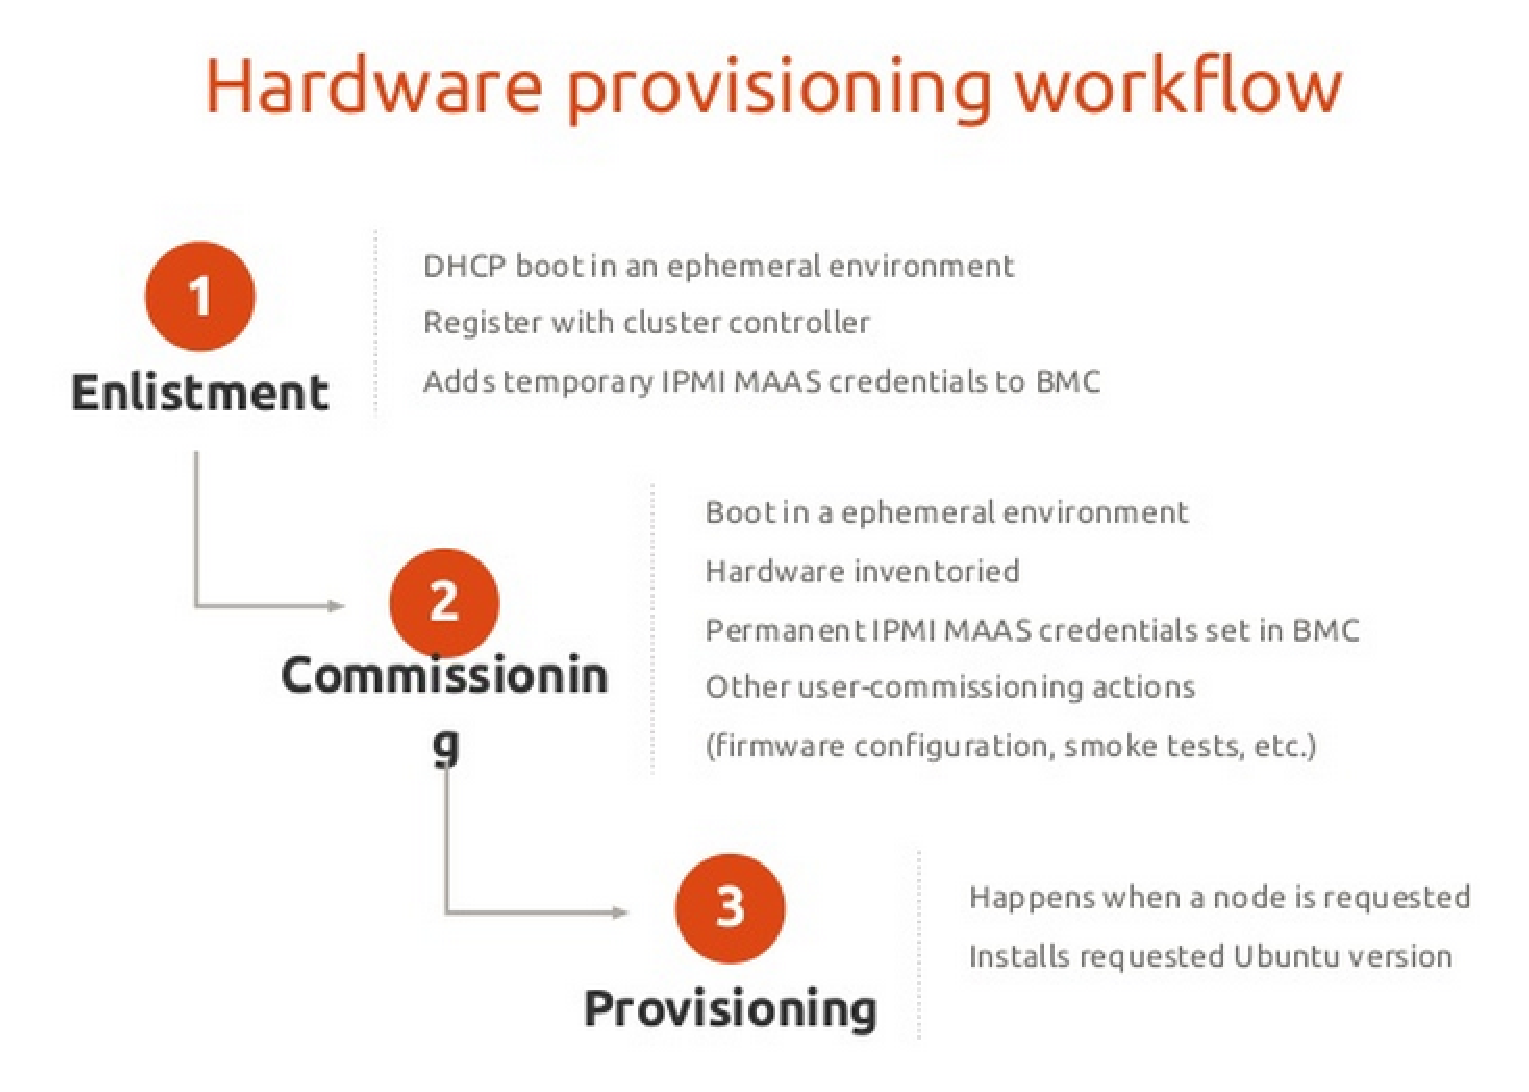
\includegraphics[height=6cm,
    angle=0]{./images/MaaS_workflow.eps}}
\caption{Enlistment, Commissioning, Deployment}
\label{fig:MaaS_workflow}
\end{figure}

The above steps can be done via a user-friendly Web UI or command-line interface
(CLI). With a simple web interface, you can  add, commission, update and recycle
your servers at will.  As your needs change, you can respond rapidly, by adding new
nodes and dynamically re-deploying them between services. When the time comes,
nodes can be retired for use outside the MaaS.  
\url{http://www.markshuttleworth.com/archives/1103}


{\bf How to turn on/off a remote machines}? There are different supported
protocols:  IPMI/iLO, Sentry Switch CDU's, or even virsh. 
By default, we expect that all the machines being controlled by MAAS have
IPMI/iLO cards. Note that MAAS not only handles physical machines, it can also handle Virtual
Machines, hence the virsh power management type. However, you will have to
manually configure the details in order for MAAS to manage these virtual
machines and turn them on/off automatically.

MAAS will attempt to auto-detect and auto-configure your IPMI/iLO cards during
the Enlistment and Commissioning processes. Once the machines are  Accepted into
MAAS (after enlistment) they will be turned on automatically and they will be
Commissioned  (that is if IPMI was discovered and configured correctly).
This also means that every time a machine is being deployed, they will be turned
on automatically.


\subsection{Do I need MAAS?}

You probably SHOULD use MAAS if any or all of the following statements are true:
\begin{verbatim}
You are trying to manage many physical servers.
You want to deploy services with the minimum fuss.
You need to get the most from your resources.
You want things to work, repeatably and reliably.
\end{verbatim}

You don't need MAAS if any or all of these statements are true
\begin{verbatim}
You don't need to manage physical hardware
You relish time spent in the server room
You like trying to set up complicated, critical services without any help
\end{verbatim}
\url{https://maas.ubuntu.com/docs/orientation.html}

\subsection{Versions}
\label{sec:MaaS_version}

While MaaS has been around for a couple of years now, it's under active
development and a lot has changed both under the hood and in the user
interface.  

Once you have installed MaaS, to check the version
\begin{verbatim}
$> apt-cache policy maas

maas:
  Installed: 1.5.4+bzr2294-0ubuntu1.3
  Candidate: 1.5.4+bzr2294-0ubuntu1.3
  Version table:
 *** 1.5.4+bzr2294-0ubuntu1.3 0
        500 http://us.archive.ubuntu.com/ubuntu/ trusty-updates/main amd64 Packages
        100 /var/lib/dpkg/status
     1.5.4+bzr2294-0ubuntu1.2 0
        500 http://security.ubuntu.com/ubuntu/ trusty-security/main amd64 Packages
     1.5+bzr2252-0ubuntu1 0
        500 http://us.archive.ubuntu.com/ubuntu/ trusty/main amd64 Packages

\end{verbatim}
\url{http://askubuntu.com/questions/470575/how-to-find-out-what-versions-of-maas-maas-dns-and-maas-dhcp-from-terminal}
\url{https://launchpad.net/~maas-maintainers/+archive/ubuntu/stable}

The script
\begin{verbatim}
 maas-import-isos
\end{verbatim}
is obsolete since Ubuntu 12.04, and is replaced by \verb!maas-import-pxe-files!
with its own configuration fie. The old script, while still there, will call to
the new script.
\url{https://code.launchpad.net/~jtv/maas/packaging-remove-maas-import-isos/+merge/119666}

\textcolor{blue}{\bf MaaS 1.4 was released with Ubuntu 13.10}
\begin{itemize}
  \item LLDP data collection on each node.
\begin{verbatim}
//lldp:chassic/lldp:id[@type="mac"]/text() = "20:4e:7f:94:2e:10"
\end{verbatim}

  \item Curtin installer is used, in replace of old Debian Installer process.
\begin{verbatim}
use-fastpath-installer
\end{verbatim}
tag to a node.

  \item more extensible templates for DHCP, power control, PXE and DNS.
  
  \item improved MaaS CLI support: user can manage their SSH keys and API
  credentials via \verb!maas-cli! tool
  
  \item Django 1.5 is used (check Python book)
  
  \item support HP Moonshot systems, as any other hardware. HP Moonshort System
  is a new world's first software-defined server platform to provide a high
  I/O throughput system, without needing a compute-intensive machine.
  
  HP Moonshot 1500 Chasssis has 45 hot-plug servers (single-server), or
  quad-server (180 servers per chassis). A hot-plug server is an integrated
  system with compute (x86, ARM, or accelerator), storage. They are
  interconnected via dual low-latency switches (45x1Gb downlinks).
  \url{http://h10032.www1.hp.com/ctg/Manual/c03728406.pdf} 
  
  MaaS can power manage HP Moonshot, and user need to manually specify the iLO
  credentials before the enlistment process begins
\begin{verbatim}
maas_moonshot_autodetect.py
\end{verbatim}
template under 
\begin{verbatim}
/etc/maas/templates/commissioning-user-data/snippets/
\end{verbatim}
\end{itemize}
\url{http://maas.ubuntu.com/docs/changelog.html\#id31}

\textcolor{blue}{\bf MaaS 1.5 was released in Ubuntu 14.04}
\begin{itemize}
  \item support multiple managed network interfaces on a single cluster
  \url{http://maas.ubuntu.com/docs/networks.html\#networks}
  
  A MaaS node can also be connected to additional networks, e.g. for your
  production workload, internet access, internal communication, or system-level
  application or application-level management tasks. MaaS does not need to
  manage these networks, but it is useful for MaaS to be aware of them. Then, we
  can provide more informations so that MaaS can do the allocation better.
  
  Example: as MaaS to allocate a node that
  \begin{itemize}
    \item must be connected to the staging network (for test application)
    \item need to share a network with a given other node (for faster
    communication)
    \item should be connected to the DMZ network (for security)
    \item can't be housed on the 'Houston' network (for resilience)
    \item has to be connected to a particular VLAN (for software-defined
    networking)
  \end{itemize}
  
  If you use virtual networks, each must have a different VLAN tag in the range
  0x001 to 0xffe (1 to 4094) inclusive. Non-virtual networks have no tag, and
  you can have as many of these as you want.  
  
  \item support defining Physical Zones (or Zones), i.e. a group of nodes.
  A physical zone should represent: it could be a server rack, a room, a data
  centre, machines attached to the same UPS, or a portion of your network. 
  Zones are most useful when they represent portions of your infrastructure. But
  you could also use them simply to keep track of where your systems are
  located. 
   
  
  Admin can define Zones. Once defined, API clients can use the zone name as
  acquisition constraints for new node allocations.
  \url{http://maas.ubuntu.com/docs/physical-zones.html}
  
  \item Hardware Enablement (HWE) Kernels (Sect.\ref{sec:HWE-kernels}): MaaS can
  fetch and user hardware enablement kernels. This allows MaaS to work with
  newer hardware which is released after the release of the given MaaS and
  Ubuntu.
  
  \url{http://maas.ubuntu.com/docs/hardware-enablement-kernels.html}
  
  \item A new project \verb!maas-test! was created: we can put a piece of
  hardware through MaaS's test suite to see if it's suitable for use in MaaS
  
  \item IPMI handling improvement
  
  \item The resource download configuration is now in a new file
 \begin{verbatim}
 /etc/maas/bootresources.yaml
 \end{verbatim}
 on each MaaS cluster controller. The new file will be pre-configured based on
 images that are already present on the cluster. This change also enables end-users to provide their own simplestreams data and
 thusly their own custom images.
 
 \textcolor{red}{OBSOLETE}: using this file 
 \begin{verbatim}
 /etc/maas/bootresources.yaml
 \end{verbatim}
 on each cluster controller is obsolete in MaaS 1.5.2 (Ubuntu 12.04), and is completely removed from MaaS
 1.6.  The sources list is now stored centrally on the MaaS region controller
 and passed to the cluster controller when the job to download boot resources is started. The
 script
 \begin{verbatim}
 /usr/sbin/maas-import-pxe-files
 \end{verbatim}
 
   \item support Seamicro 15000 hardware: power control and API-based enlistment
   
   \item support Intel AMT: power control
   
   \item can configure an upstream DNS: to use bind daemon's forwarders' option.
   
   \item can detect foreign DHCP server: and show you if any other DHCP servers
   are active on the networks that are on the cluster controller.
   
   \item show commissioning results on the web UI
   
   \item \textcolor{red}{MaaS CLI are renamed}: 
   \begin{itemize}
     \item \verb!maas! is renamed to \verb!maas-region-admin!
     \item \verb!maas-cli! is renamed to \verb!maas!
   \end{itemize}
 
\end{itemize}

\textcolor{blue}{\bf MaaS 1.6} 
\begin{itemize}
  \item IP addresses overhaul: a major change with totally different IP
  allocation.
  
  We can define static IP range for cluster interfaces configuration that is
  separate DHCP server's dynamic range: Any node in use by a user will receive
  an IP address from this static range that is guaranteed not to change during
  its allocated time.
  
  In the future release, it only give DNS entries to static IPs.
  \url{http://maas.ubuntu.com/docs1.6/api.html\#ip-addresses}
  
  \item DNS entries changed from 'CNAME record in MaaS 1.5 to 'A' record in this
  version.
  
  \item completely remove \verb!bootresources.yaml! (see MaaS 1.5). To manage a
  boot source
  \begin{verbatim}
DELETE /api/1.0/nodegroups/{uuid}/boot-sources/{id}/
  \end{verbatim}
  \url{http://maas.ubuntu.com/docs1.6/api.html\#boot-source}
  
  \item the fast installer is the default to replace the old Debian Installer
  for the new enlisted nodes. The existing nodes can keep using their default
  installer.
  \url{https://launchpad.net/curtin}
  
\end{itemize}

\textcolor{blue}{\bf Ubuntu 14.04.1 with MaaS 1.7}
\begin{itemize}
  \item non-Ubuntu O/S are fully support: CentOS, Windows OS, SuSE
  
  \item support deploy custom images: can be uploaded via the API. 
  
  We can deploy other Ubuntu flavors, e.g. Ubuntu Desktop.
  
  \item \verb!maas-proxy! is the default proxy instead of
  \verb!squid-deb-proxy!.
  
  \item support IPv6: we can deploy Ubuntu nodes that have IPv6
  
  \item node-specific log: major events on MaaS nodes can be logged, e.g. power
  changes, deployments and any failures.
  
  \item RPC connections:

  \item remove 2 components: Celery and RabbitMQ
  
  Celery is used in production systems to process millions of tasks a day.
  However, it is not considered to suit MaaS project's requirement due to its
  fire-and-forgot mechanism. A custom communication mechanism between the region
  controller and cluster controllers is developed. The new mechanism is
  bidirectional and allowed the complex interactions to take place that are
  required as part of the robustness improvements. This allows a constant
  connection is maintained.
  
  
  
  \item MaaS 1.7.1 : not yet released
  \begin{itemize}
    \item 
  \end{itemize}
  
  \item MaaS 1.7.2: not yet released
  \begin{itemize}
    \item 
  \end{itemize}
  
  \url{https://launchpad.net/maas/1.7}
\end{itemize}
\url{https://launchpad.net/maas/+milestones}

\subsection{Structure of a Ubuntu MaaS cluster}
\label{sec:MaaS_structure}

The key components of the MaaS softwares are
\begin{itemize}
  \item Region controller
  \item Cluster controller
  \item A few or thousands of nodes
\end{itemize}
\url{https://maas.ubuntu.com/docs/orientation.html}

\begin{figure}[hbt]
  \centerline{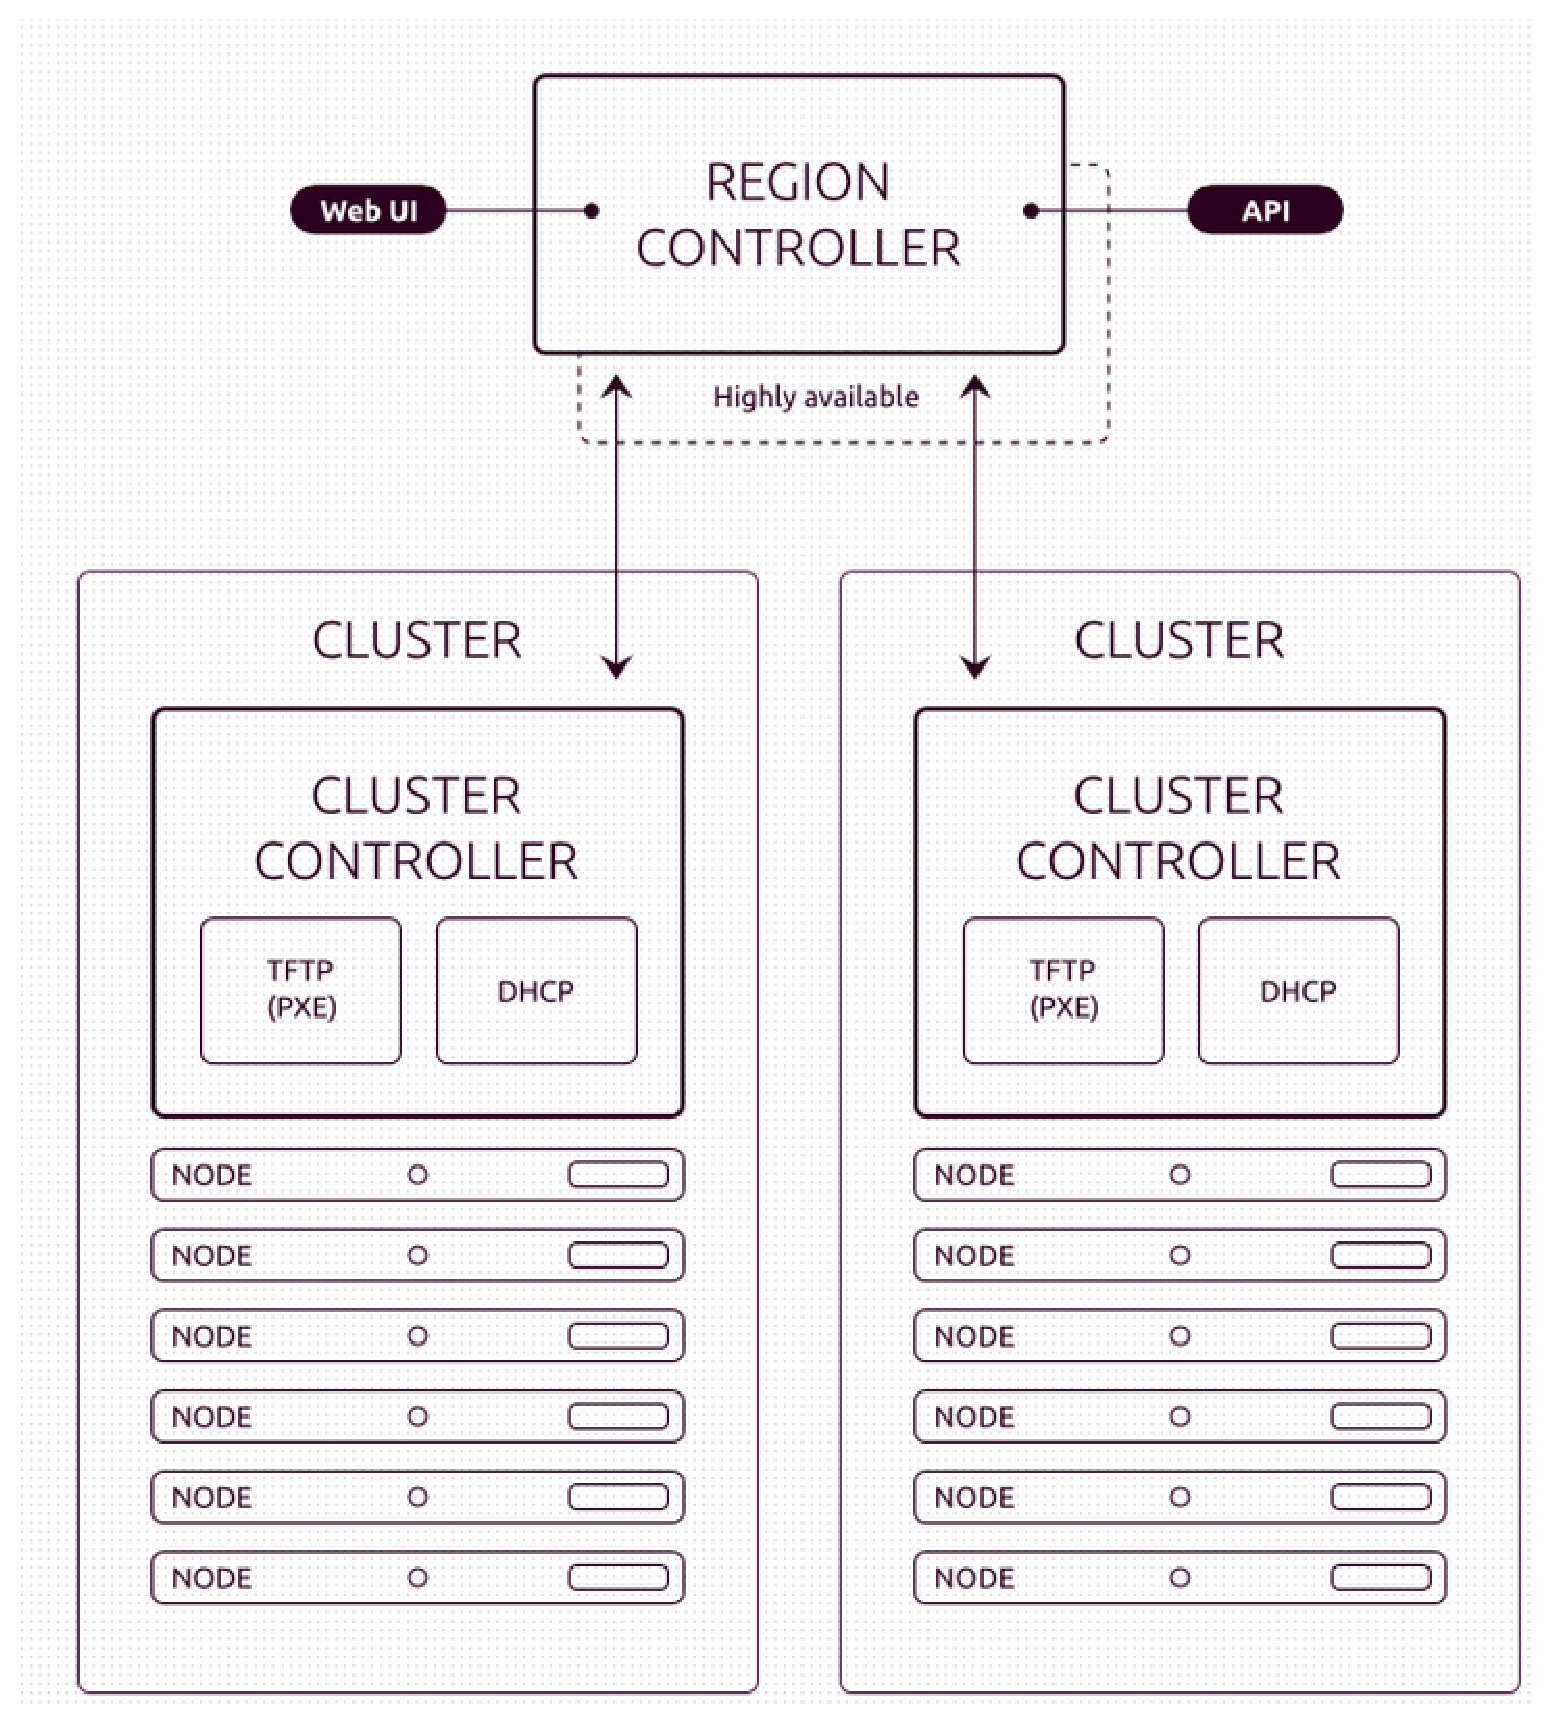
\includegraphics[height=6cm,
    angle=0]{./images/MaaS_region_controller_cluster_controller.eps}}
\caption{MaaS: region controller with Web UI and remote API}
\label{fig:MaaS_region_controller_cluster_controller}
\end{figure}

In a big system, the Ubuntu MaaS configuration has separated MaaS Regional
Controller Server and MaaS Cluster Controller Server. It is only worth having
multiple region controllers if you need to organise your nodes into different
subnets. 
\begin{itemize}
  \item  
  A region controller associates with one or more
cluster controllers, each of which is responsible for contacting the region
controller itself and announcing its presence.

The region controller provides Web UI and remote API to access the different
associated MaaS clusters.

 \item The MaaS Controller Server could control
several networks using each network adapter of the MaaS Server, so we can expand
the local cloud network.

  \item The nodes are the computers you manage using MAAS. 
\end{itemize}

However in a small local cloud implementation we could install both services in
a single server, Fig.\ref{fig:MaaS_minimum}. For the convenience of small setups
(and the development environment), the first cluster controller to connect to
the region controller becomes the 'master' nodegroup, and if the cluster
connects from the same host, it is automatically accepted. \textcolor{red}{There
is always at least one cluster controller in MaaS} (known as {\bf NodeGroup} in
the code) which is known as the master.
 

\begin{figure}[hbt]
  \centerline{\includegraphics[height=5cm,
    angle=0]{./images/MaaS_minimum.eps}}
  \caption{Minimal MaaS system}
\label{fig:MaaS_minimum}
\end{figure}

REQUIREMENT: 
\begin{enumerate}
  \item MaaS server
  \begin{itemize}
  \item Three NIC cards: connect to the Internet with 1 NIC, and the private
  network on the other
  \item Ubuntu Server
  \end{itemize} 
  
  \item MaaS node
  \begin{itemize}
    \item Two NIC cards
    \item 
  \end{itemize} 
\end{enumerate}

\textcolor{red}{\bf STEP 1}: Before any of MaaS's features can be used for the
first time, you must have a MaaS region controller. We can either install MaaS region controller
+ cluster controller at the same time
(Sect.\ref{sec:MaaS_install_region-controller_and_cluster-controller}), or
install MaaS region controller separately
(Sect.\ref{sec:install_MaaS_region-controller}). Once we have MaaS region
controller installed, we need to create the admin account
(Sect.\ref{sec:configure_MaaS_region-controller}), and download the boot images
(for the first times only) to the region controller
(Sect.\ref{sec:MaaS_download-boot-images}).\url{http://maas.ubuntu.com/docs1.5/install.html}

\textcolor{red}{\bf STEP 2}: we install MaaS cluster controller. If we used
Sect.\ref{sec:MaaS_install_region-controller_and_cluster-controller}, then
cluster controller has already been installed on the same with the region
controller. If we want to install on a separate machine, install Ubuntu server
version on that machine, and run
\begin{verbatim}
sudo apt-get install maas-cluster-region
\end{verbatim} 
We then need to tell the region controller to accept the cluster controller
(Sect.\ref{sec:configure_MaaS-cluster-controller}).

\textcolor{red}{\bf STEP 3}: Configure MaaS cluster controller to be able to
detect the new nodes easily. This requires a DHCP server and DNS server
\begin{itemize}
  \item DHCP server: a daemon to assign IP to the new MaaS nodes in a given
  cluster controller (Sect.\ref{sec:DHCP}).
  
  \item DNS server: to perform name resolution, e.g. map hostname to IP.
\end{itemize}

IP of the nodes it manage in an automatically
manner.
There are three possible ways to assign IP to MaaS nodes
\url{https://maas.ubuntu.com/docs/cluster-configuration.html\#cluster-configuration}

\begin{enumerate}
  \item The MaaS cluster controller also control the IP assignment via
  MaaS DHCP server \verb!maas-dhcp! and MaaS name resolution server via
  \verb!maas-dns! (Sect.\ref{sec:MaaS_maas-dhcp})

%   
%   MaaS suggests to use its own DHCP server \verb!maas-dhcp!.
% \textcolor{blue}{DHCP is needed in order for MaaS to boot and control nodes.}
% There are
% two ways to assign IP, static or dynamic. To assign a dynamic IP to a machine,
% we need a DHCP server which manages the IP assignment .
  
  
  \item The MaaS cluster controller control IP assignment via
  \verb!maas-dhcp! only  (Sect.\ref{sec:MaaS_maas-dhcp})
  
  
  \item MaaS interface depend on an external DHCp server that is configured
  manually. This is not recommended.
  
   Configure existing DHCP server to work with MaaS
  (Sect.\ref{sec:MaaS_use-existing-DHCP-server}).
  
  If you don't want to use MaaS DHCP server, we need to alter the configuration of
the existing DHCP server to allow MaaS to enlist and control nodes
automatically.
Use DHCP for the first network interface that is connected to your router/modem.
After the installation you can set static IP on the second network interface for
the local cloud infrastructure subnet.
  
  \item Existing DHCP server that you does not have access to control
\end{enumerate}




If you only have 1 network interface on the MAAS server: don't use DHCP, use
static local IP: 191.168.100.1 / 255.255.255.0. The best configuration is that
you have 2 network interface on the MAAS server:


Then, we can add one or more MaaS nodes to the MaaS server later on
(Sect.\ref{sec:MaaS_node_install}). Each node in the cluster should be attached
to one of these networks. (In addition, a node can be attached to any number of
networks that are not managed by MaaS.) See how to configure a private network
(Sect.\ref{sec:private_network}).

% To bootstrap a MaaS environment, you need to have MaaS installed in one machine
% by
% \begin{itemize}
%   \item install MaaS as part of a fresh Ubuntu server install: use CD, and
%   choose ``Multiple Server install with MaaS''. This will install both the MaaS
%   region controller and cluster controller services on the same machine
%   (Sect.\ref{sec:install_MaaS_region-controller})
%   
%   \item on an existing Ubuntu server system, then install the MaaS package
%   (Sect.\ref{sec:MaaS_install_existing-Ubuntu-server})
%   
%   If we want to install MaaS region controller and cluster controller on two
%   separate machines, follow this approach.
% \end{itemize}

% Also, we need a MaaS region controller, to be able to control remotely via a Web
% UI and/or remote API (Sect.\ref{sec:install_MaaS_region-controller}).


% \subsection{MaaS Ubuntu region controller and/or cluster controller}
% 
\subsection{Install MaaS (region controller + cluster controller)}
\label{sec:MaaS_install_region-controller_and_cluster-controller}
%\label{sec:install_MaaS_region-controller}

 
NOTE: The following packages can be installed on a single server
\begin{itemize}
  \item \verb!maas!: seed cloud setup (includes both region controller and
  cluster controller)
  \item \verb!maas-region-controller! : include web UI, API and database
  \item \verb!maas-cluster-controller! : control a group of nodes, including
  DHCP management.
  
  \item \verb!maas-dhcp!, \verb!maas-dns!: required when managing DHCP/DNS.
\end{itemize}

{\bf IMPORTANT}: When MaaS region or Cluster controller going down, it won't
affect the provisioned servers (existing machines that are allocated and
running are not affected), only that new servers will not be acquired,
provisioned or enlisted. Also, if only a cluster that went down then only that
cluster's machines are affected. 
\url{http://askubuntu.com/questions/346048/does-a-maas-region-or-cluster-controller-going-down-mean-the-provisioned-servers}


{\bf Option 1}:   Here, we describe steps to install MaaS (region controller +
cluster controller) during Ubuntu installation using Ubuntu server 14.04.1
(Check to know which version of MaaS - Sect.\ref{sec:MaaS_version}). 
\begin{itemize}
  \item Multiple server install with MaaS
  \item enter hostname, e.g. hadu01
  \item Enter MaaS installation part. There are two options: (1) create a new
  MaaS on this server, (2) specify MaaS by name or address.
  
  We choose the first one, as this is the MaaS server.
  
  \item Enter admin username for the actual server that MaaS will be running on,
  NOT the MaaS program admin user. 
  
  \item Does the server need a HTTP proxy to access the outside world?
  
  Leave it blank, or configure in the form
\begin{verbatim}
http://[[user] [:pass]@]host[:port]/"
\end{verbatim}
  
  \item {\bf Configure MaaS region controller}: this is the IP address of the
  MaaS regional controller. This is simply the address of the server you're
  trying to setup, if the server will be used as the MaaS region controller.
  Then, we can access the MaaS region controller server via a web-interface
\begin{verbatim}
http://192.168.1.10/MAAS
\end{verbatim}
Make sure the address being used is in the same network as the MaaS clients.    
  
  The MaaS API is also a set of command line tools too. Everything you can do
  with the webpage you can do with a command line tool and a lot more
  (Sect.\ref{sec:MaaS_command-line}).
  I personally don't use the command line tools because it is easy to mess things
  up and not be able to see exactly what I did.  
  
%   information that the MaaS
%   region/cluster controller will use to tell the MaaS nodes how to reach the
%   cluster controller.  
  \url{http://askubuntu.com/questions/458481/install-maas-before-i-install-maas}
  
\end{itemize}

{\bf Option 2}: Here, we have the option to install MaaS region controller on
one machine and cluster controller on another machine using two separate
commands. Of course, if we run them on the same machines, both will be installed
and run on a single server.
\begin{verbatim}
// install both 
sudo apt-get install maas

// install region controller
sudo apt-get install maas-region-controller

// install cluster controller
sudo apt-get install maas-cluster-controller

\end{verbatim} 

Result:
\begin{verbatim}
The following extra packages will be installed:
  maas-cli maas-cluster-controller maas-common maas-dns maas-region-controller
  maas-region-controller-min python-django-maas python-maas-client
  python-maas-provisioningserver
Suggested packages:
  ipmitool libvirt-bin amtterm
The following packages will be upgraded:
  maas-cli maas-cluster-controller maas-common maas-dhcp maas-dns
  maas-region-controller maas-region-controller-min python-django-maas
  python-maas-client python-maas-provisioningserver
10 upgraded, 0 newly installed, 0 to remove and 145 not upgraded.
\end{verbatim}

Confirm packages installed
\begin{verbatim}
$> dpkg --get-selections | grep maas

maas                                            install
maas-cli                                        install
maas-cluster-controller                         install
maas-common                                     install
maas-dhcp                                       install
maas-dns                                        install
maas-region-controller                          install
maas-region-controller-min                      install
python-django-maas                              install
python-maas-client                              install
python-maas-provisioningserver                  install

\end{verbatim}


It is recommended to use up-to-date MaaS from Canonical cloud archive.
The archive contains important fixes and new features that is not always
available in the Ubuntu archive.
\begin{verbatim}
// old Ubuntu (to install add-apt-repository)
sudo apt-get install python-software-properties
// since Ubuntu 11.10, a symlink is created
//  apt-add-repository --> add-apt-repository

// from Ubuntu 13.10
sudo apt-get install software-properties-common
 
 // then we run (only on Ubuntu 12.04)
 // not able to work on Ubuntu 14.04 
sudo add-apt-repository cloud-archive:tools

  // Ubuntu 14.04+
sudo add-apt-repository ppa:maas-maintainers/stable

sudo apt-get update  
\end{verbatim}
\url{http://askubuntu.com/questions/38021/how-to-add-a-ppa-on-a-server}
Error:
\url{http://askubuntu.com/questions/549341/cant-add-cloud-archivetools-to-repository} 
{\tiny
\begin{verbatim}
// error on Ubuntu 14.04

Traceback (most recent call last):
  File "/usr/bin/add-apt-repository", line 163, in <module>
    if not sp.add_source_from_shortcut(shortcut, options.enable_source):
  File "/usr/lib/python3/dist-packages/softwareproperties/SoftwareProperties.py", line 727, in add_source_from_shortcut
    (deb_line, file) = shortcut.expand(codename=self.distro.codename)
  File "/usr/lib/python3/dist-packages/softwareproperties/cloudarchive.py", line 98, in expand
    if codename not in (MAP[self.caname]['release'],
KeyError: 'release'
\end{verbatim}
}
\url{https://launchpad.net/~maas-maintainers/+archive/ubuntu/stable}

You may be asked
\begin{verbatim}
Configuration file '/etc/maas/pserv.yaml'
 ==> Modified (by you or by a script) since installation.
 ==> Package distributor has shipped an updated version.
   What would you like to do about it ?  Your options are:
    Y or I  : install the package maintainer's version
    N or O  : keep your currently-installed version
      D     : show the differences between the versions
      Z     : start a shell to examine the situation
 The default action is to keep your current version.
*** pserv.yaml (Y/I/N/O/D/Z) [default=N] ?

\end{verbatim}

The changes are
\begin{verbatim}
--- /etc/maas/pserv.yaml        2015-01-22 16:38:33.587707545 -0600
+++ /etc/maas/pserv.yaml.dpkg-new       2014-12-09 12:51:30.000000000 -0600
@@ -19,15 +19,6 @@
   # reporter:
   reporter: "maas-pserv"

-## Message broker configuration (optional, not currently used).
-#
-broker:
-  # host: "localhost"
-  # port: 5673
-  # username: <current user>
-  # password: "test"
-  # vhost: "/"
-
 ## TFTP configuration.
 #
 tftp:
@@ -39,5 +30,5 @@

   # port: 69
   ## The URL to be contacted to generate PXE configurations.
-  generator: http://192.168.1.148/MAAS/api/1.0/pxeconfig/
+  # generator: http://localhost/MAAS/api/1.0/pxeconfig/
\end{verbatim}

\begin{verbatim}
Installing new version of config file /etc/maas/pserv.yaml ...
Installing new version of config file /etc/sudoers.d/99-maas-sudoers ...
Installing new version of config file /etc/logrotate.d/maas-cluster-controller ...

AH00558: apache2: Could not reliably determine the server's fully qualified domain name, using 127.0.1.1. Set the 'ServerName' directive globally to suppress this message

Removing obsolete conffile /etc/init/maas-cluster-celery.conf ...
Removing obsolete conffile /etc/init/maas-pserv.conf ...

Configuration file '/etc/maas/maas_local_settings.py'
 ==> Modified (by you or by a script) since installation.
 ==> Package distributor has shipped an updated version.
   What would you like to do about it ?  Your options are:
    Y or I  : install the package maintainer's version
    N or O  : keep your currently-installed version
      D     : show the differences between the versions
      Z     : start a shell to examine the situation
 The default action is to keep your current version.
*** maas_local_settings.py (Y/I/N/O/D/Z) [default=N] ?

\end{verbatim}


The changes are
\begin{verbatim}
--- /etc/maas/maas_local_settings.py    2015-01-22 16:38:25.263707336 -0600
+++ /etc/maas/maas_local_settings.py.dpkg-new   2014-12-09 12:51:30.000000000 -0600
@@ -4,7 +4,7 @@
 # Default URL specifying protocol, host, and (if necessary) port where
 # systems in this MAAS can find the MAAS server.  Configuration can, and
 # probably should, override this.
-DEFAULT_MAAS_URL = "http://192.168.1.148/MAAS"
+DEFAULT_MAAS_URL = "http://maas.internal.example.com/"

 # Absolute path to the directory static files should be collected to.
 STATIC_ROOT = '/usr/share/maas/web/static/'
@@ -23,12 +23,6 @@
 # Use the package's files to serve RaphaelJS.
 RAPHAELJS_LOCATION = '/usr/share/javascript/raphael/'

-# RabbitMQ settings.
-RABBITMQ_HOST = 'localhost'
-RABBITMQ_USERID = 'maas_longpoll'
-RABBITMQ_PASSWORD = '1HNQAh63bFMPE4q6kpps'
-RABBITMQ_VIRTUAL_HOST = '/maas_longpoll'
-
 # See http://docs.djangoproject.com/en/dev/topics/logging for
 # more details on how to customize the logging configuration.
 LOGGING_LEVEL = 'INFO'
@@ -43,7 +37,10 @@
     'handlers': {
         'log': {
             'class': 'logging.handlers.RotatingFileHandler',
-            'filename': '/var/log/maas/maas.log',
+            # DO NOT point this file at /var/log/maas/maas.log; MAAS now
+            # uses syslog to log to that file, and pointing the Django
+            # log output to it will clobber the syslog output.
+            'filename': '/var/log/maas/maas-django.log',
             'formatter': 'simple',
         },
     },
@@ -77,13 +74,19 @@
 }

 # Database access configuration.
+from psycopg2.extensions import ISOLATION_LEVEL_READ_COMMITTED
+
+
 DATABASES = {
     'default': {
         # 'postgresql_psycopg2', 'postgresql', 'mysql', 'sqlite3' etc.
         'ENGINE': 'django.db.backends.postgresql_psycopg2',
         'NAME': 'maasdb',
         'USER': 'maas',
-        'PASSWORD': 'g9jsjAO7Non3',
+        'PASSWORD': 'maas',
         'HOST': 'localhost',
+        'OPTIONS': {
+            'isolation_level': ISOLATION_LEVEL_READ_COMMITTED,
+        },
     }
 }
\end{verbatim}


\subsection{Install MaaS region controller}
\label{sec:install_MaaS_region-controller}

% In either way, MaaS will include all of the PXE, DHCP, DNS and other services it
% needs to work. 

We run
\begin{verbatim}
// install region controller
sudo apt-get install maas-region-controller

sudo dpkg-reconfigure maas-region-controller
\end{verbatim}
and make sure to select the IP address that is used for PXE and provisioning
(i.e. in the same network with the MaaS nodes). This is not the IP of the
router/modem.
\begin{verbatim}
192.168.1.10
\end{verbatim}

Next step: configure MaaS region controller
(Sect.\ref{sec:configure_MaaS_region-controller})



% \subsubsection{Install MaaS by command line}
% \label{sec:MaaS_install_existing-Ubuntu-server}




\subsection{Configure MaaS region controller (Web UI, remote API)}
\label{sec:configure_MaaS_region-controller}

After you install MaaS region controller
(Sect.\ref{sec:MaaS_install_region-controller_and_cluster-controller} or
Sect.\ref{sec:install_MaaS_region-controller}), if we try to open MaaS via Web
UI, and dialog will display an error message, Fig.\ref{fig:MaaS_no_admin}.

\begin{figure}[hbt]
  \centerline{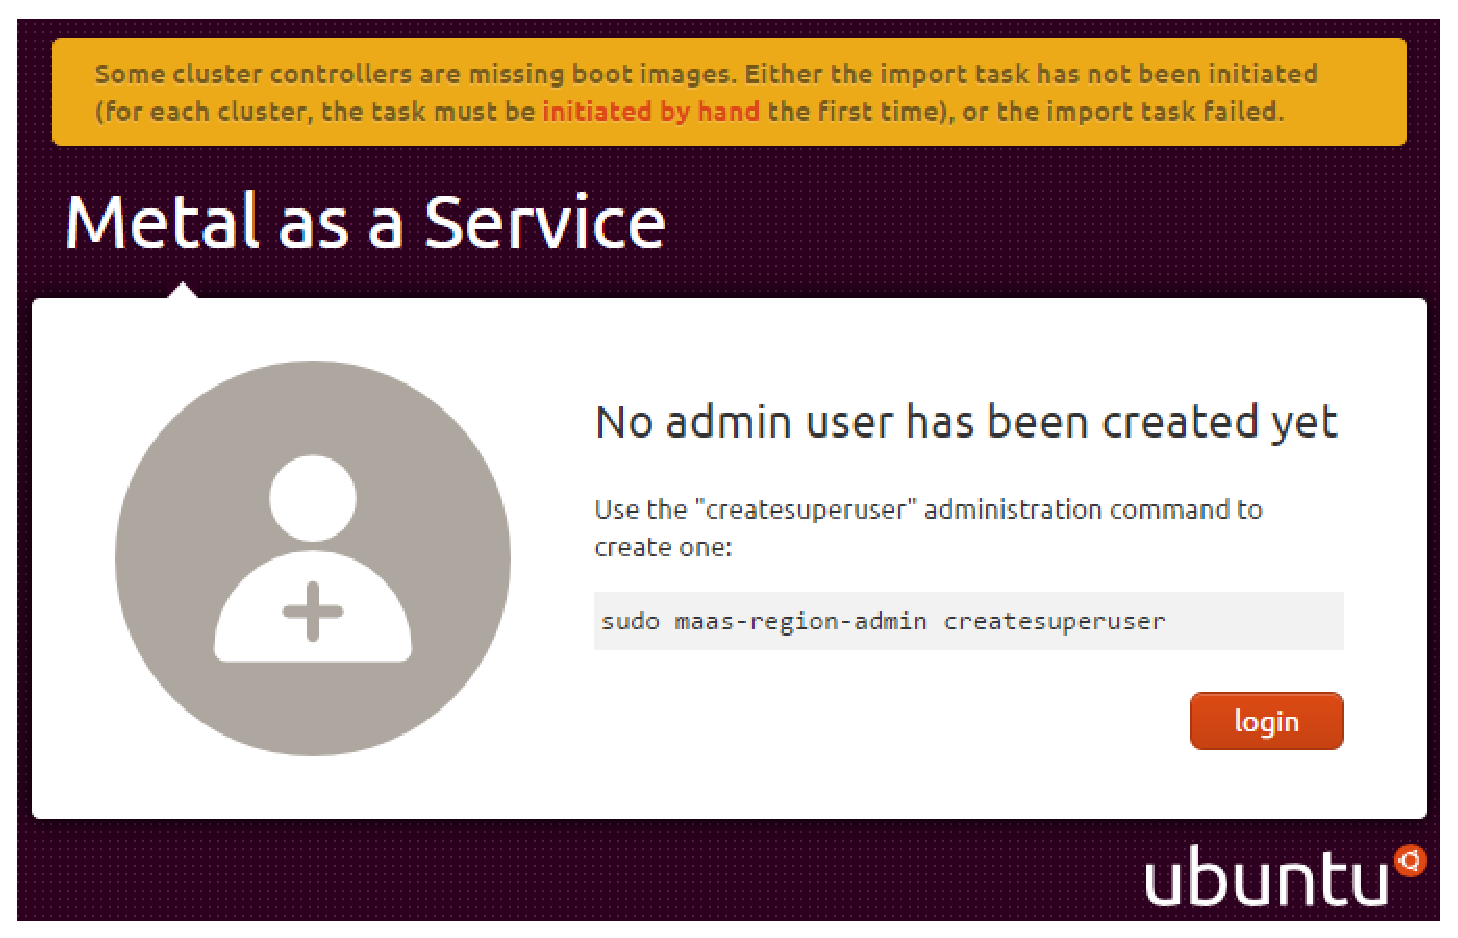
\includegraphics[height=4cm,
    angle=0]{./images/MaaS_no_admin.eps}}
\caption{Login error to MaaS: need a user-account to login}
\label{fig:MaaS_no_admin}
\end{figure}

We need to create an admin user to login to the Web UI to control the MaaS
(Sect.\ref{sec:MaaS_user-account}). Activate API key for shell cocmmand,
assuming the admin account is named 'root'
\begin{verbatim}
sudo maas-region-admin apikey --username=root>maasapikey

cat maasapikey
\end{verbatim}
The file named \verb!maasapikey! is stored in the current folder.

So, we have two options to control MaaS: (1) web UI, (2) command line.

{\bf Web UI}: Now, from another machine, use the web browser to connect to MaaS regional
server
\begin{verbatim}
http://192.168.1.10/MAAS
 
 // from outside: port forward 192.168.100.123 to 192.168.1.10
http://192.168.100.123/MAAS
\end{verbatim}
You may see the error
\begin{verbatim}
No admin user has been created
\end{verbatim}
You may need to enable port forwarding on the router
(Sect.\ref{sec:port_forwarding}).

To use HTTPS for secure access to MaaS web UI/API, we need to turn on SSL
support in Apache
\begin{verbatim}
sudo a2enmod ssl
\end{verbatim}
then, ensure Apache config file 
\begin{verbatim}
/etc/maas/maas-http.conf
\end{verbatim}
file is included \verb!/etc/apache2/conf.d/! folder, and edit
\begin{verbatim}
/etc/maas/maas_local_settings.py
\end{verbatim}
and change \verb!DEFAULT_MAAS_URL! so that it uses https instead of http.
Finally, we restart Apache
\begin{verbatim} 
sudo service apache2 restart
\end{verbatim}
NOTICE: The default SSL certificate is insecure, we need to generate our own and
then edit \verb!/etc/apache2/conf.d/maas-http.conf! file to set the location to
the new certificate.



{\bf Command line}: login to MaaS session with the session name is
\verb!my-maas-session! (you can name it anything)
\begin{verbatim}
sudo maas login my-maas-session http://172.17.172.1/MAAS/api/1.0 -|cat ~/maasapikey
\end{verbatim}
Then we check that the session is logged-in properly
\begin{verbatim}
sudo maas my-maas-session node-groups list
\end{verbatim}


Reconfigure MaaS region controller
\begin{verbatim}
  //NOTE: rerun these commands if you change the IP address
  //      of the MaaS server
sudo dpkg-reconfigure maas-region-controller
\end{verbatim}

\subsection{Download boot images (first time)}
\label{sec:MaaS_download-boot-images}

Since MaaS 1.7, the boot images are stored in the region controller's database,
from where the cluster controllers will synchronize and pull images to the
cluster's local disk, Fig.\ref{fig:MaaS_Web_UI_maas1.7}. This process is
automatic and MAAS will check for and download new Ubuntu images every hour. 

\begin{figure}[hbt]
  \centerline{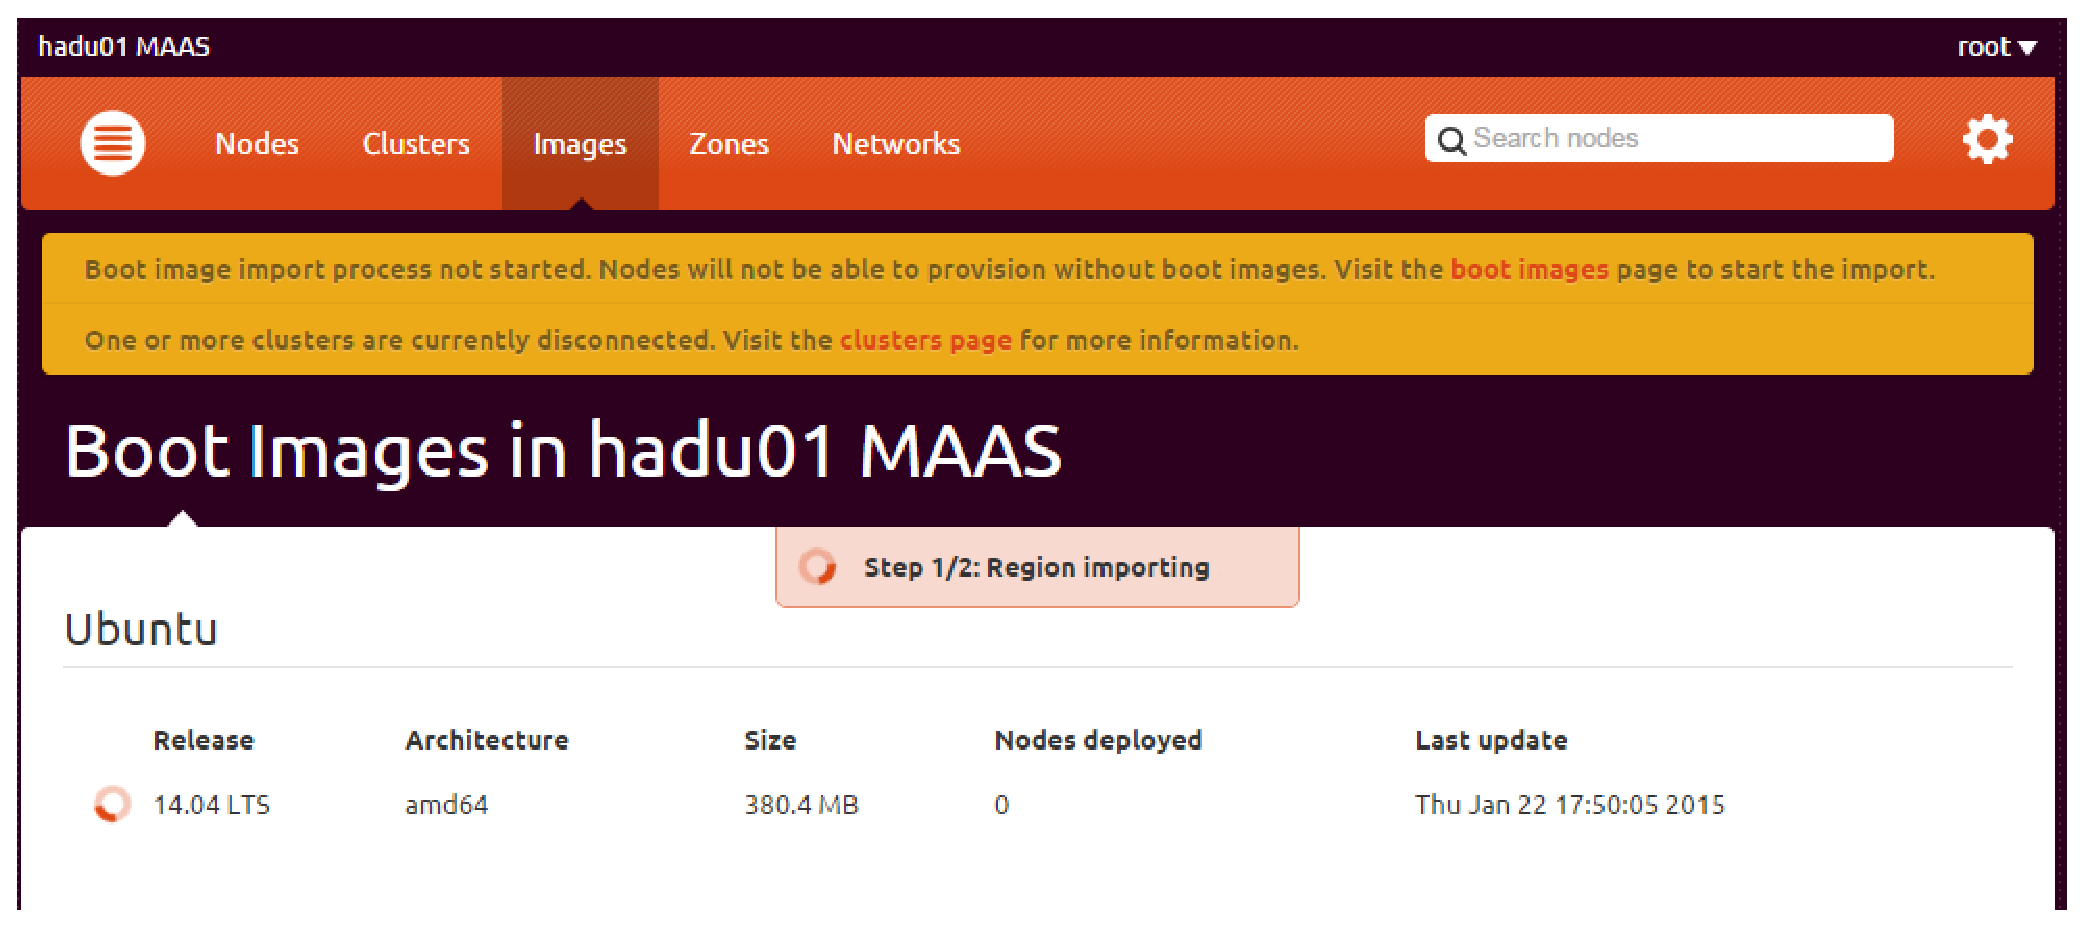
\includegraphics[height=6cm,
    angle=0]{./images/MaaS_Web_UI_maas1.7.eps}}
\caption{A new {\bf Images} tab is added in MaaS 1.7 as the mangement of boot
images is transferred to the region controller}
\label{fig:MaaS_Web_UI_maas1.7}
\end{figure}


If there is no available boot images on the region controller, you will see this
message, and you won't be able to add new MaaS nodes to the cluster.
\begin{verbatim}
Some cluster controllers are missing boot images. Either the import task has not
been initiated (for each cluster, the task must be initiated by hand the first
time), or the import task failed.
\end{verbatim}
MAAS will check for and download new Ubuntu images once a week. However, you'll
need to download them manually the first time. 


There are two ways to import:
\begin{itemize}
  \item via the Web UI
  \item via the remote API
  \item via \verb!maas-import-pxe-files! Python script 
  
\begin{verbatim}
sudo maas-import-pxe-files
sudo /usr/sbin/maas-import-pxe-files
\end{verbatim}
\end{itemize}
We recommend triggering manual imports through the UI or API over the
maas-import-pxe-files script. However there may be circumstances where you might
prefer the command-line script, in which case there are several differences you
need to be aware of: 


{\tiny
\begin{verbatim}
$>sudo maas-import-pxe-files

2015-01-22 15:10:46,511 INFO Importing boot resources.
2015-01-22 15:11:20,250 INFO Inserting file boot-kernel (tag=b146783134b20619cd92c998e567c959d6ca2687b7609fb952f5740b3348e907, size=5806368).
2015-01-22 15:11:20,250 INFO Inserting file di-kernel (tag=d4fc2ba26cad96f4360cb36f04c26b2f50dceee9413c206431148b87e4958909, size=5800024).
2015-01-22 15:11:20,250 INFO Inserting file boot-initrd (tag=d9f59b43a593b4b7bb04dc1329e29c9dfca86dd0d8f9f06ce0966bc184dfe763, size=24887599).
2015-01-22 15:11:20,250 INFO Inserting file di-initrd (tag=71fb5916ad1ee63a1de85e2ed623400201be76566704b7a94503b46637412f44, size=21268557).
2015-01-22 15:11:20,250 INFO Inserting file boot-kernel (tag=7c140615232c1165310df1742559b09d1f6616ebf52826457c20c6a37cad2de5, size=5457776).
2015-01-22 15:11:20,251 INFO Inserting file di-kernel (tag=741724f0e357738f3e14ddafa586e677f8da5a7bf14ff81fc464baa18ea47424, size=5460184).
2015-01-22 15:11:20,251 INFO New root image: /var/lib/maas/boot-resources/cache/root-image-b29afeeec5421a53dc28bf5c6c67f40544136f5dfcdd4b520da159c58d9e130e.
2015-01-22 15:13:51,831 INFO Converting root tarball: /var/lib/maas/boot-resources/cache/root-tgz-b29afeeec5421a53dc28bf5c6c67f40544136f5dfcdd4b520da159c58d9e130e.
Thu, 22 Jan 2015 15:13:51 -0600: converting /var/lib/maas/boot-resources/cache/root-image-b29afeeec5421a53dc28bf5c6c67f40544136f5dfcdd4b520da159c58d9e130e to /var/lib/maas/boot-resources/cache/root-tgz-b29afeeec5421a53dc28bf5c6c67f40544136f5dfcdd4b520da159c58d9e130e
Thu, 22 Jan 2015 15:13:51 -0600: copying contents of /var/lib/maas/boot-resources/cache/root-image-b29afeeec5421a53dc28bf5c6c67f40544136f5dfcdd4b520da159c58d9e130e in /var/lib/maas/boot-resources/cache/root-image-b29afeeec5421a53dc28bf5c6c67f40544136f5dfcdd4b520da159c58d9e130e to /var/lib/maas/boot-resources/cache/root-tgz-b29afeeec5421a53dc28bf5c6c67f40544136f5dfcdd4b520da159c58d9e130e
Thu, 22 Jan 2015 15:14:16 -0600: finished. wrote to /var/lib/maas/boot-resources/cache/root-tgz-b29afeeec5421a53dc28bf5c6c67f40544136f5dfcdd4b520da159c58d9e130e
2015-01-22 15:14:16,228 INFO Inserting file boot-initrd (tag=9265ba86349370d5a011a1f48af66c9c3ae0e9bf519388a652db10239824b4b8, size=20972396).
2015-01-22 15:14:45,891 INFO Inserting file di-initrd (tag=aced2e916e9654e2dcd05c406d2da46e69b789eb9e900e4057695f5835c2454a, size=19181380).
2015-01-22 15:15:04,015 INFO Inserting file boot-kernel (tag=dcdb75633cbf79e372ad2779bf61fe6ea1321e0e57f6f9f66785db7de8db8324, size=5814832).
2015-01-22 15:15:17,856 INFO Inserting file di-kernel (tag=2eedc84677c1598bfe01171174bfd499b9c700f8df5d7563418cdac3239c35ad, size=5800848).
2015-01-22 15:15:31,134 INFO New root image: /var/lib/maas/boot-resources/cache/root-image-5514563cb36a09eac04e58f75cd11856765b048f03440c0ec751d82fd2b6dd6b.
2015-01-22 15:19:55,904 INFO Converting root tarball: /var/lib/maas/boot-resources/cache/root-tgz-5514563cb36a09eac04e58f75cd11856765b048f03440c0ec751d82fd2b6dd6b.
Thu, 22 Jan 2015 15:19:55 -0600: converting /var/lib/maas/boot-resources/cache/root-image-5514563cb36a09eac04e58f75cd11856765b048f03440c0ec751d82fd2b6dd6b to /var/lib/maas/boot-resources/cache/root-tgz-5514563cb36a09eac04e58f75cd11856765b048f03440c0ec751d82fd2b6dd6b
Thu, 22 Jan 2015 15:19:55 -0600: copying contents of /var/lib/maas/boot-resources/cache/root-image-5514563cb36a09eac04e58f75cd11856765b048f03440c0ec751d82fd2b6dd6b in /var/lib/maas/boot-resources/cache/root-image-5514563cb36a09eac04e58f75cd11856765b048f03440c0ec751d82fd2b6dd6b to /var/lib/maas/boot-resources/cache/root-tgz-5514563cb36a09eac04e58f75cd11856765b048f03440c0ec751d82fd2b6dd6b
Thu, 22 Jan 2015 15:20:25 -0600: finished. wrote to /var/lib/maas/boot-resources/cache/root-tgz-5514563cb36a09eac04e58f75cd11856765b048f03440c0ec751d82fd2b6dd6b
2015-01-22 15:20:25,517 INFO Inserting file boot-initrd (tag=b14968c2335c43256180c6556ffe61fb62e2f98739b0f4f7c30c5ef29b7751fa, size=23370573).
2015-01-22 15:20:49,532 INFO Inserting file di-initrd (tag=e446a27d7ddfe1b59b7fa8a34186b14f897d194737f51ea5ce9fadeca625f06d, size=19434159).
2015-01-22 15:21:09,754 INFO Inserting file boot-kernel (tag=84e218ac3ab178da874f83c1ef67ee6a55abd9125295873162bc7d9d3d560f7a, size=5472512).
2015-01-22 15:21:22,261 INFO Inserting file di-kernel (tag=cb503643c7d7e0433edaa6a15b8b41289711574ffea1aec7344e4a63888c7992, size=5472480).
2015-01-22 15:21:41,020 INFO New root image: /var/lib/maas/boot-resources/cache/root-image-4e7d750db15f95b5b39c8382e4aefbca9ec452a5fdd208514f08bc667bf66a5f.
Thu, 22 Jan 2015 15:24:43 -0600: finished. wrote to /var/lib/maas/boot-resources/cache/root-tgz-4e7d750db15f95b5b39c8382e4aefbca9ec452a5fdd208514f08bc667bf66a5f
2015-01-22 15:24:44,083 INFO Inserting file boot-initrd (tag=a6fc73e3e4e11f6efb32b70d74a30896473ebfe90992d87ba26ab9e69d05babc, size=19889503).
2015-01-22 15:25:09,857 INFO Inserting file di-initrd (tag=c71beeb938b609fce4b803d08b737d0433b97997281e3503efc8212417af65cb, size=17518515).
2015-01-22 15:25:26,666 INFO Writing metadata and updating iSCSI targets.
2015-01-22 15:25:26,739 INFO Installing boot images snapshot /var/lib/maas/boot-resources/snapshot-20150122-151103.
2015-01-22 15:27:15,079 INFO Import done.

\end{verbatim}
}


Script content:
\begin{verbatim}
#! /usr/bin/python2.7
# -*- mode: python -*-
# Copyright 2014 Canonical Ltd.  This software is licensed under the
# GNU Affero General Public License version 3 (see the file LICENSE).

"""Import boot resources into MAAS cluster controller."""

from __future__ import (
    absolute_import,
    print_function,
    unicode_literals,
    )

str = None

__metaclass__ = type

import logging
from provisioningserver.import_images.boot_resources import (
    maaslog,
    main_with_services,
    make_arg_parser,
    NoConfigFile,
    )

logger = logging.getLogger(__name__)

if __name__ == "__main__":
    parser = make_arg_parser(__doc__)
    args = parser.parse_args()
    try:
        main_with_services(args)
    except NoConfigFile:
        maaslog.error("Config file %s not found." % args.config_file)
        raise SystemExit(1)
    except Exception:
        # logger.exception() will log the error message, followed by the
        # exception's stack trace. Using it here rather than allowing
        # the exception to kill the process unhandled means we can be
        # sure about where the exception ends up, rather than it
        # potentially vanishing.
        logger.exception("Unhandled exception; unable to continue.")
        raise SystemExit(2)
\end{verbatim}

\subsection{Configure MaaS cluster controller (nodegroup)}
\label{sec:configure_MaaS-cluster-controller}

Once we have installed MaaS cluster controller, we need to ask the region
controller to accept this cluster controller. A cluster controller controls a
nodegroup.

Below are possible status for a nodegroup
\begin{itemize}
  \item DEFAULT : the default is \verb!PENDING!
  \item PENDING : has been created and awaits approval.
  \item ACCEPTED
  \item REJECTED
\end{itemize}
\url{http://maas.ubuntu.com/docs/enum.html\#maasserver.models.NODE_STATUS}
The cluster controller control one or more network Interface, which can be 
\begin{itemize}
  \item UNMANAGED : tell the MaaS not to control the DHCP or DNS of this
  interface
  
  \item DHCP  : tell MaaS to manage DHCP only 
  \item DHCP\_AND\_DNS : 
\end{itemize}

If you see \verb!pending cluster!,
it means the cluster need to be accepted by the region controller. The first
cluster controller is called {\bf Cluster master}, by default.

\begin{figure}[hbt]
  \centerline{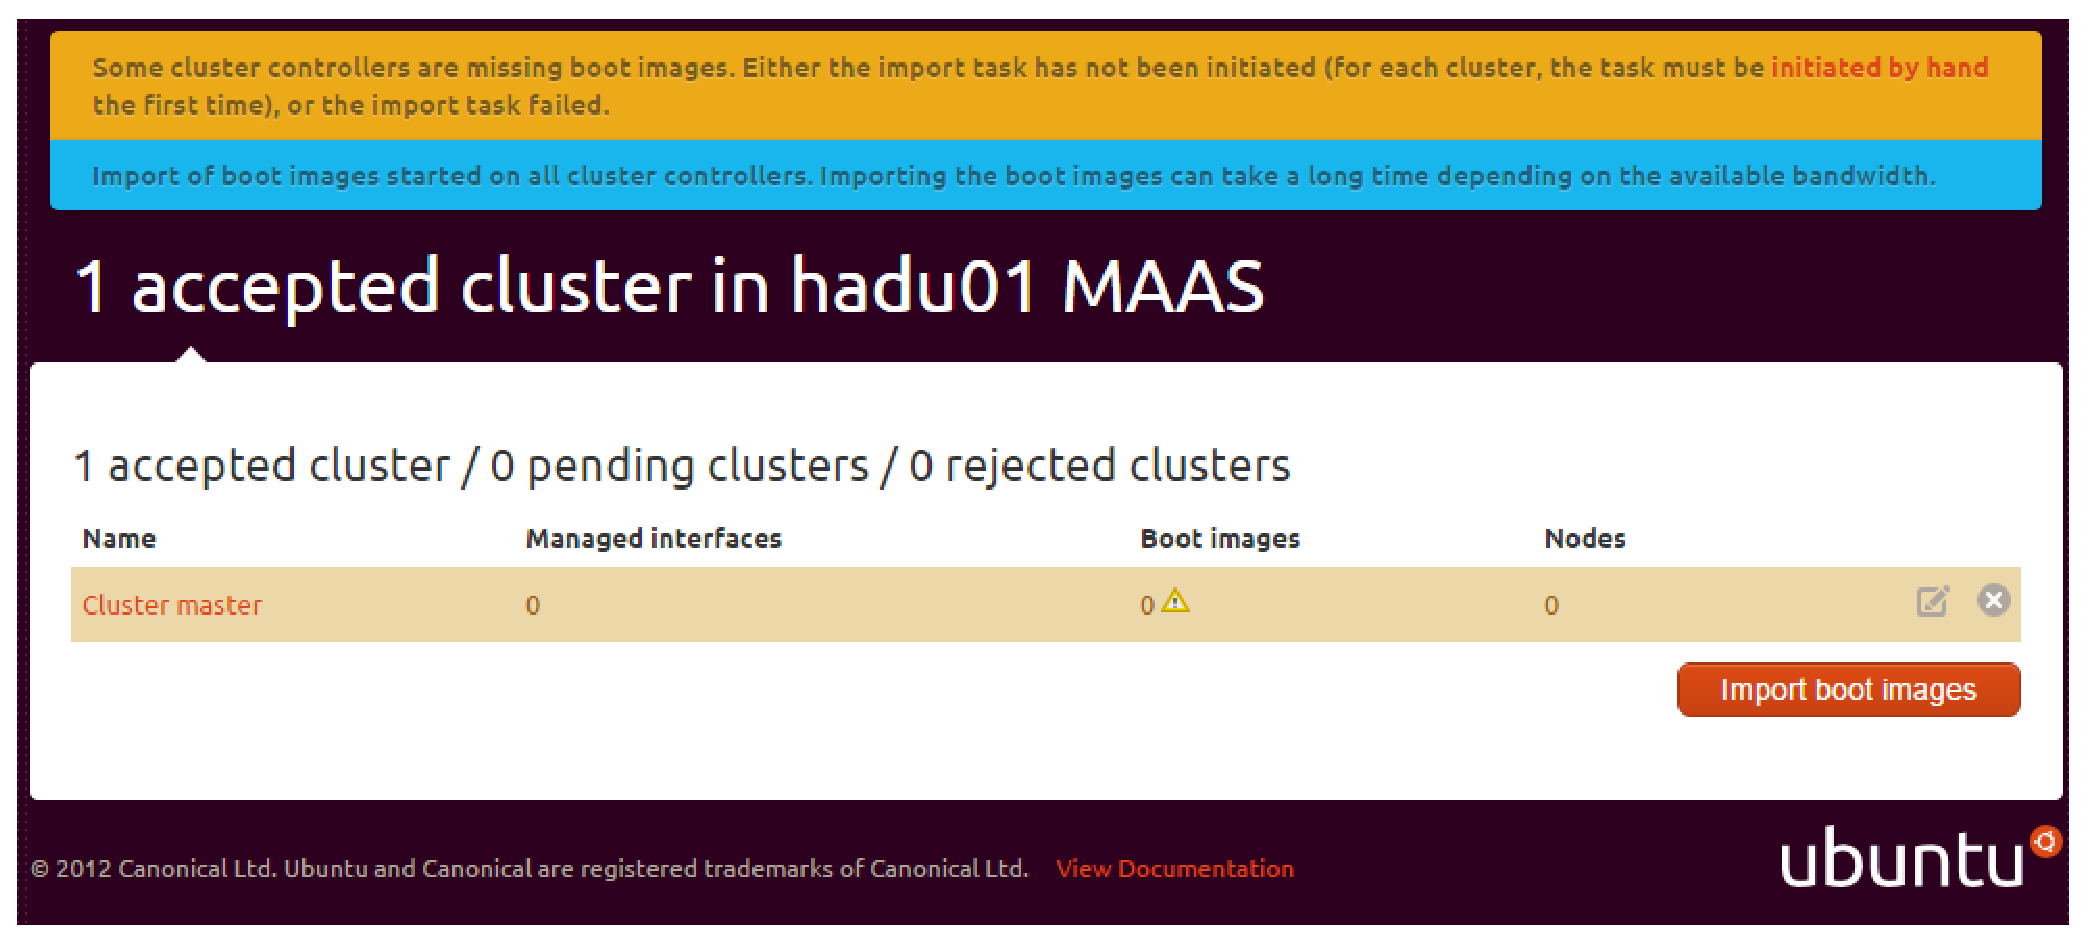
\includegraphics[height=4cm,
    angle=0]{./images/MaaS_cluster_controller.eps}}
\caption{MaaS: add a cluster controller to the region controller}
\label{fig:MaaS_cluster_controller}
\end{figure}

Whenever we make changes to the
cluster controller or region controller
\begin{verbatim}
sudo dpkg-reconfigure maas-cluster-controller 
\end{verbatim}

Example: The MaaS cluster controller has 2 Interfaces: p2p1 (public) and p3p1
(MaaS nodegroup)
\begin{verbatim}
# The primary network interface
auto p2p1
iface p2p1 inet static
  address 192.168.100.123
  netmask 255.255.255.0
  gateway 192.168.100.1
  dns-nameservers 192.168.100.70
  dns-nameservers 192.168.100.80
  dns-nameservers 192.168.100.11
auto p3p1
iface p3p1 inet static
  address 192.168.1.10
  netmask 255.255.255.0
  gateway 192.168.1.1
  dns-nameservers 192.168.1.10
\end{verbatim}



\subsection{MaaS CLI (command-line interface)}
\label{sec:MaaS_command-line}

We can work with MaaS via a web interface or a command-line interface (CLI).
This section describes the CLI.
Before the API will accept any commands from maas, you must first log in. To do
this, you need an API key for your MAAS account. A key was generated for you as
soon as your account was created, although you can still generate additional
keys if you prefer.  To check the key, we can do via Web UI
\begin{verbatim}
Click on the user's name on the top right of the Web UI
   Select Preferences
      Check MAAS KEY (one MAAS key for one session)
\end{verbatim}
or via the command line
\begin{verbatim}
// old MAAS
sudo maas-region-admin apikey <my-username>

// MAAS 1.7
sudo maas-region-admin apikey --username=<my-username>
\end{verbatim}
with \verb!<my-username>! is your username. If we login multiple sessions, we
need multiple keys.

We can now login by (1) name a profile which can be reused across command-line
invocations (as a persistent session)
\begin{verbatim}
maas login <profile-name> <MAAS_region-hostname> <key>
\end{verbatim}
Example:
\begin{verbatim}
maas login my-maas http://10.98.0.13/MAAS/api/1.0
       AWSCRMzqMNy:jjk...5e1FenoP82Qm5te2
       
sudo maas login my-session  http://192.168.1.10/MAAS/api/1.0 C8MWrsRLLzrarzNbkB:2eX7AcxTzdWeXxy2Mt:dLUxEBKyZSD9QJKgp8ZnvLj7YHUsD7Fk

You are now logged in to the MAAS server at
http://192.168.1.10/MAAS/api/1.0/ with the profile name 'my-session'.

For help with the available commands, try:

  maas my-session --help
       
\end{verbatim}

To get help
{\tiny
\begin{verbatim}
tietronix@hadu01:~$ maas my-session --help
usage: /usr/lib/python2.7/dist-packages/maascli/__main__.py my-session
       [-h] COMMAND ...

Issue commands to the MAAS region controller at http://192.168.1.10/MAAS/api/1.0/.

optional arguments:
  -h, --help            show this help message and exit

drill down:
  COMMAND
    account             Manage the current logged-in user.
    boot-images         Manage the collection of boot images.
    boot-resource       Manage a boot resource.
    boot-resources      Manage the boot resources.
    boot-source         Manage a boot source.
    boot-source-selection
                        Manage a boot source selection.
    boot-source-selections
                        Manage the collection of boot source selections.
    boot-sources        Manage the collection of boot sources.
    commissioning-script
                        Manage a custom commissioning script.
    commissioning-scripts
                        Manage custom commissioning scripts.
    file                Manage a FileStorage object.
    files               Manage the collection of all the files in this MAAS.
    ipaddresses         Manage IP addresses allocated by MAAS.
    license-key         Manage a license key.
    license-keys        Manage the license keys.
    maas                Manage the MAAS server.
    network             Manage a network.
    networks            Manage the networks.
    node-group          Manage a NodeGroup.
    node-group-interface
                        Manage a NodeGroupInterface.
    node-group-interfaces
                        Manage the collection of all the NodeGroupInterfaces
                        in this MAAS.
    node-groups         Manage the collection of all the nodegroups in this
                        MAAS.
    node                Manage an individual Node.
    node-mac            Manage a Node MAC address.
    node-macs           Manage MAC addresses for a given Node.
    node-results        Read the collection of NodeResult in the MAAS.
    nodes               Manage the collection of all the nodes in the MAAS.
    sshkey              Manage an SSH key.
    sshkeys             Manage the collection of all the SSH keys in this
                        MAAS.
    sslkey              Manage an SSL key.
    sslkeys             Operations on multiple keys.
    tag                 Manage a Tag.
    tags                Manage the collection of all the Tags in this MAAS.
    users               Manage the user accounts of this MAAS.
    zone                Manage a physical zone.
    zones               Manage physical zones.

This is a profile.  Any commands you issue on this profile will
operate on the MAAS region server.

The command information you see here comes from the region server's
API; it may differ for different profiles.  If you believe the API may
have changed, use the command's 'refresh' sub-command to fetch the
latest version of this help information from the server.

\end{verbatim}
}

List of all commands:
\url{https://maas.ubuntu.com/docs/maascli.html}


%\subsection{Reconfigure MaaS system}


\subsection{DHCP server: maas-dhcp}
\label{sec:MaaS_maas-dhcp}


\begin{figure}[hbt]
  \centerline{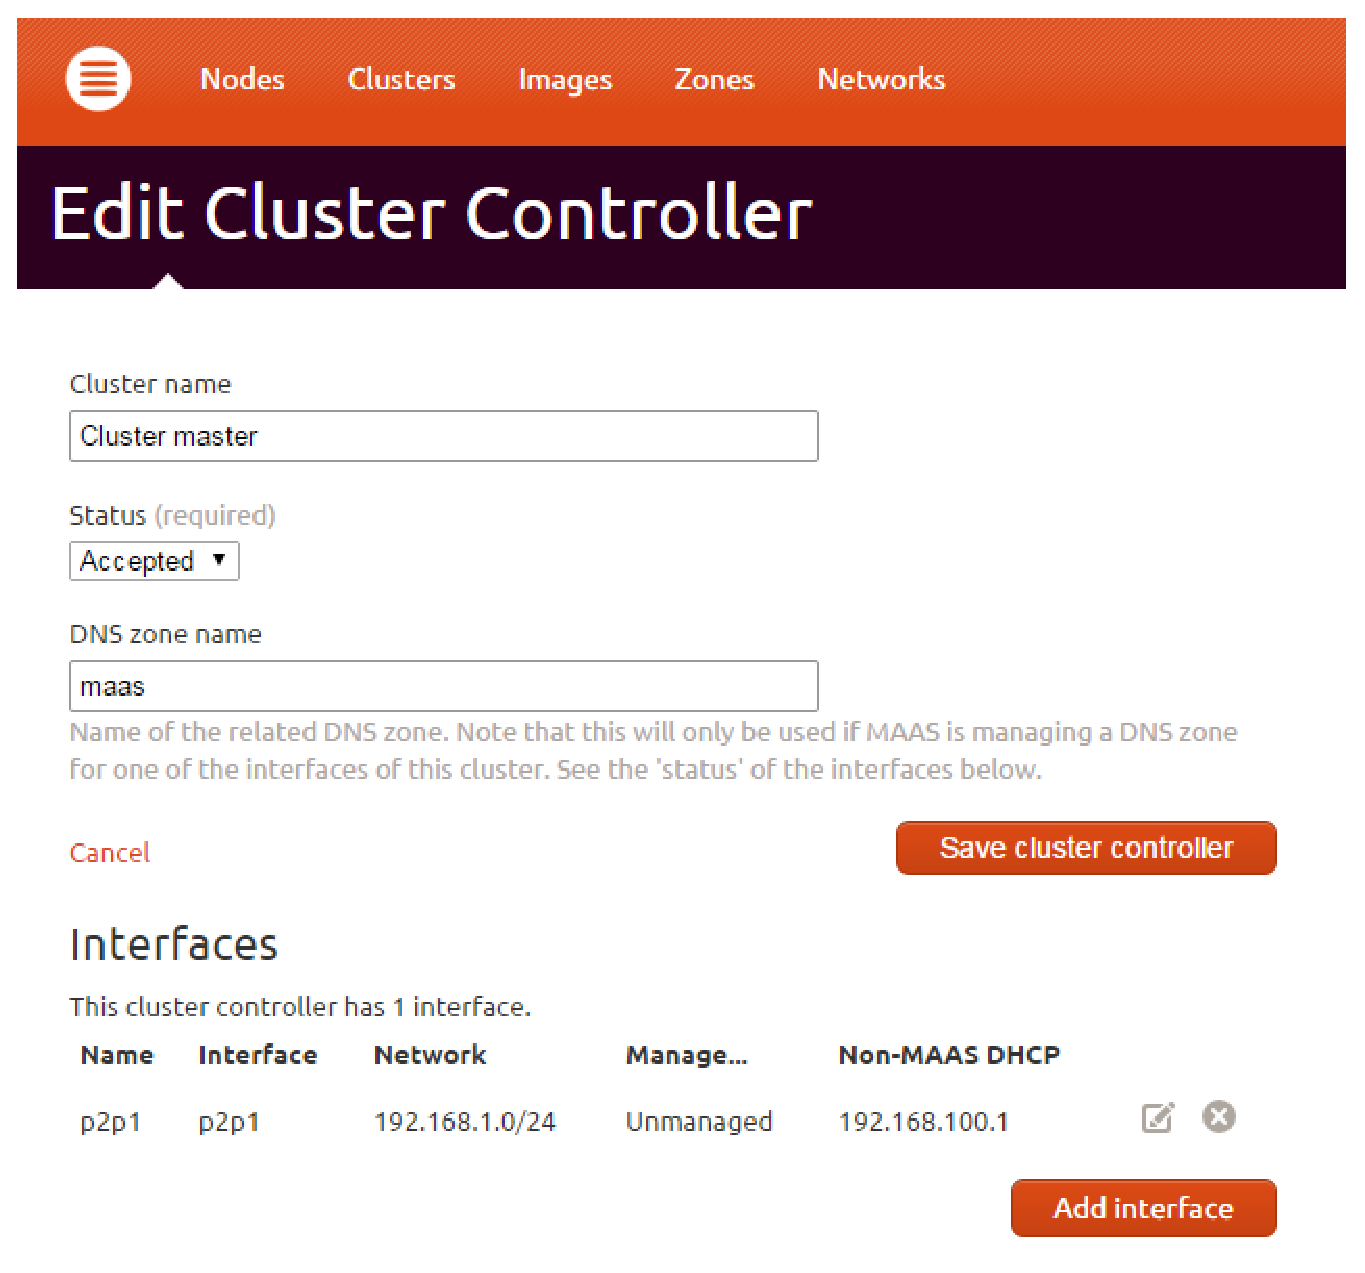
\includegraphics[height=6cm,
    angle=0]{./images/MaaS_cluster-network_interface.eps}}
  \centerline{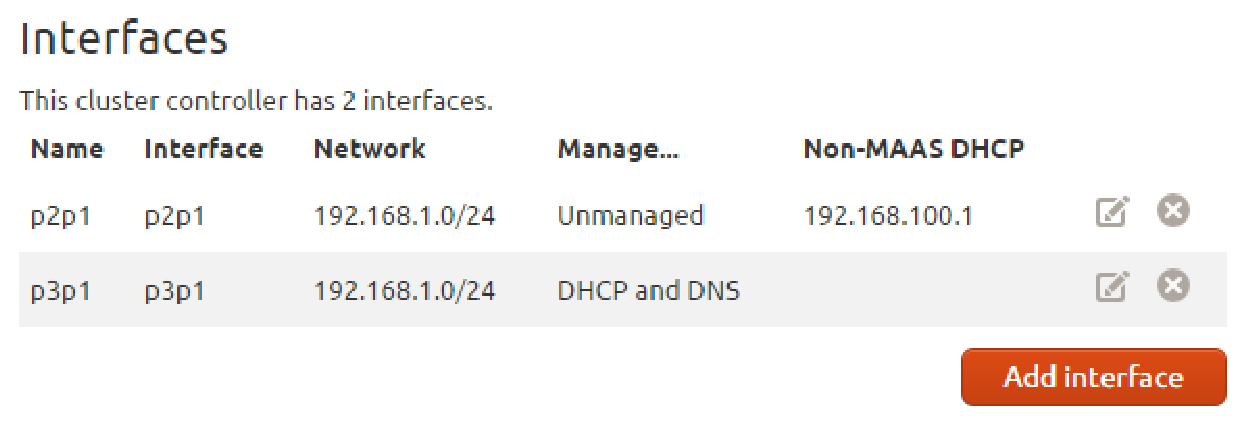
\includegraphics[height=3cm,
    angle=0]{./images/MaaS_managed_interface.eps}}
\caption{(A) Only unmanaged interface; (B) With Managed interface by the MaaS
cluster controller}
\label{fig:MaaS_cluster-network_interface}
\end{figure}


% You can choose whichever DHCP server you prefer but for this guide we'll use
% \verb!dnsmasq! via the maas-dhcp package.

We need to install \verb!maas-dhcp! and \verb!maas-dns! packages
explicitly
\begin{verbatim}
dpkg -l maas-dhcp maas-dns

sudo apt-get install maas-dhcp maas-dns
\end{verbatim}
The cluster controller has one Interface (which can be Ethernet or Infiniband)
connecting to a router or switch from that the MaaS nodes will be connected. In
order for the cluster controller to be able to manage nodes through this
Interfaces, the nodes must be on the same subnet as the cluster controller's
Interface. At first, the IP of the cluster controller's interface should be
configured static. Explain: \verb!p2p1! is the interface to the public network,
\verb!p3p1! is the interface to the cloud network 
\begin{verbatim}
auto p2p1
iface p2p1 inet static
  address 192.168.100.123
  netmask 255.255.255.0
  gateway 192.168.100.1
  dns-nameservers 192.168.100.70
  dns-nameservers 192.168.100.80
  dns-nameservers 192.168.100.11
auto p3p1
iface p3p1 inet static
  address 192.168.1.10
  netmask 255.255.255.0
  gateway 192.168.1.1
  dns-nameservers 192.168.100.70
  dns-nameservers 192.168.100.80
  dns-nameservers 192.168.100.11
\end{verbatim}

In Fig.\ref{fig:MaaS_cluster-network_interface}(A), the cluster controller has
one Unmanaged Interface. We need to add an Interface to be managed by MaaS
DHCP, Fig.\ref{fig:MaaS_cluster-network_interface}(B).
There is also an option to leave the network unmanaged. Use this for networks
where you don't want to manage any nodes. Or, if you do want to manage nodes but
don't want the cluster controller to serve DHCP, you may be able to get by
without it

% Here is the information when we decide to use MaaS DHCP server, then you may need to know how to configure a private network
% (Sect.\ref{sec:private_network}).  

% dnsmasq might already be installed, however, it is not configured to work with MaaS. In order to install and/or configure it, enter the following:
% \begin{verbatim}
% sudo apt-get install maas-dhcp
% \end{verbatim}

\begin{itemize}
  \item Name: e.g. \verb!cloud_01!
  
  \item Interface: p3p1, eth1

Choose \verb!p3p1!
  
  \item Management: Unmanaged, DHCP and DNS, DHCP only.
  
  Choose DHCP and DNS.
  
  \item IP : the IP of the MaaS cluster controller (must be the same subnet
  with the MaaS nodes)
  
\begin{verbatim}
192.168.1.10
\end{verbatim}

  \item subnet mask: of the region under this MaaS cluster controller
\begin{verbatim}
255.255.255.0
\end{verbatim}
  
  \item broadcast IP: It is usually something along the lines and ending in 255.
\begin{verbatim}
192.168.1.255
\end{verbatim}
  
  \item Router IP: The IP of the router for your subnet as part of the MaaS
  region (it is the gateway). This is the IP to the larger Internet here.
  
\begin{verbatim}
192.168.1.10
\end{verbatim}

There is a bug fix reported to make Router IP optional.
\url{https://bugs.launchpad.net/maas/+bug/1334325} A workaround solution is to
remove the line 
\begin{verbatim}
 option routers {{dhcp_subnet['router_ip']}};
\end{verbatim}
from the file
\begin{verbatim}
/etc/maas/templates/dhcp/dhcpd.conf.template
\end{verbatim}
  
  \item DHCP dynamic IP range low value:  the start address for where a MAAS
  controller will begin handing out IP addresses to other clients. 
  
  \item DHCP dynamic IP range high value
  
  \item Static IP range low value
  
  \item Static IP range high value
\end{itemize}
\url{http://askubuntu.com/questions/455527/whats-the-correct-maas-dhcp-configuration}


The information above is saved into \verb!/etc/maas/dhcpd.conf! file
\begin{verbatim}
option path-prefix code 210 = text; #RFC5071
subnet 192.168.1.0 netmask 255.255.255.0 {
       if option arch = 00:0E {
          filename "pxelinux.0";
          option path-prefix "ppc64el/";
       } elsif option arch = 00:07 {
          filename "bootx64.efi";
       } elsif option arch = 00:0C {
          filename "bootppc64.bin";
       } else {
          filename "pxelinux.0";
       }
       interface "p3p1";
       ignore-client-uids true;
       option subnet-mask 255.255.255.0;
       option broadcast-address 192.168.1.255;
       option domain-name-servers 192.168.1.10;
       option domain-name "maas";
       option routers 192.168.1.1; //we can remove it here
       option ntp-servers ntp.ubuntu.com;
       range dynamic-bootp 192.168.1.2 192.168.1.100;
       class "PXE" {
          match if substring (option vendor-class-identifier, 0, 3) = "PXE";
          default-lease-time 30;
          max-lease-time 30;
       }
}

\end{verbatim}
The content of this file is templated in 
\begin{verbatim}
 /etc/maas/templates/dhcp/dhcpd.conf.template
\end{verbatim}
%and copy to \verb!/etc/maas/dhcpd.conf! file.

IMPORTANT: A single cluster controller can manage more than one network, each
from a different cluster interface. This may help you scale your cluster to larger
numbers of nodes, or it may be a requirement of your network architecture. 

NOTE: Installation \verb!maas-dhcp! log.
\begin{verbatim}
Considering dependency proxy for proxy_http:
Module proxy already enabled
Module proxy_http already enabled
Module expires already enabled
Module wsgi already enabled

squid-deb-proxy start/running, process 8302
Setting up maas-dns (1.5.4+bzr2294-0ubuntu1.2) ...
Setting up maas-cli (1.5.4+bzr2294-0ubuntu1.2) ...
Setting up maas-dhcp (1.5.4+bzr2294-0ubuntu1.2) ...

maas-dhcp-server stop/pre-start, process 8386
Setting up maas-cluster-controller (1.5.4+bzr2294-0ubuntu1.2) ...
Installing new version of config file /etc/sudoers.d/99-maas-sudoers ...
Installing new version of config file /etc/maas/templates/dhcp/dhcpd.conf.template ...

maas-pserv start/running, process 8630
maas-cluster-celery start/running, process 8664
Setting up maas-region-controller (1.5.4+bzr2294-0ubuntu1.2) ...

 Restarting PostgreSQL 9.3 database server     
 Restarting web server apache2   
 Restarting message broker rabbitmq-server     
 
Changing password for user "maas_longpoll" ...
...done.
Changing password for user "maas_workers" ...
...done.

Synced:
 > django.contrib.auth
 > django.contrib.contenttypes
 > django.contrib.sessions
 > django.contrib.sites
 > django.contrib.messages
 > django.contrib.staticfiles
 > piston
 > south

Not synced (use migrations):
 - maasserver
 - metadataserver

(use ./manage.py migrate to migrate these)
Running migrations for maasserver:
- Nothing to migrate.
 - Loading initial data for maasserver.
Installed 1 object(s) from 1 fixture(s)
Running migrations for metadataserver:
- Nothing to migrate.
 - Loading initial data for metadataserver.
Installed 1 object(s) from 1 fixture(s)
 * Restarting web server apache2                                                                                                                                                                                                                                                                                                                                    [ OK ]
squid-deb-proxy stop/waiting
squid-deb-proxy start/running, process 9592
maas-txlongpoll stop/waiting
maas-txlongpoll start/running, process 9683
maas-region-celery stop/waiting
maas-region-celery start/running, process 9772
 
\end{verbatim}

\subsection{DHCP server: existing DHCP server}
\label{sec:MaaS_use-existing-DHCP-server}

If you use a different DHCP server, we need to alter the configuration to allow
MaaS to enlist and control nodes explicitly. How to configure depends on what
software being used as the DHCP server. At the very least, the \verb!filename!
option should be set to \verb!pxelinux.0!. 

Example: ISC DHCP server
\begin{verbatim}
subnet 192.168.122.0 netmask 255.255.255.0 {
    filename "pxelinux.0";
    option subnet-mask 255.255.255.0;
    option broadcast-address 192.168.122.255;
    option domain-name-servers 192.168.122.136;
    range dynamic-bootp 192.168.122.5 192.168.122.135;
}
\end{verbatim}
When doing this, leave the cluster controller's interface in the "unmanaged"
state.

\url{http://maas.ubuntu.com/docs1.5/configure.html\#manual-dhcp}


\subsection{DNS: maas-dns}
\label{sec:MaaS_maas-dns}

\verb!maas-dns! uses bind9 DNS server (Sect.\ref{sec:bind9}). Thus, when we
install \verb!maas-dns!
\begin{verbatim}
sudo apt-get install maas-dns
\end{verbatim}

A folder is created inside /etc/bind
\begin{verbatim}
/etc/bind/maas
\end{verbatim}
This is a DNS zone, and then it modifies the content of two files
under \verb!/etc/bind! folder.
\begin{verbatim}
named.conf.local:include "/etc/bind/maas/named.conf.maas";
named.conf.options:include "/etc/bind/maas/named.conf.options.inside.maas";
\end{verbatim}

When using a third party tool such as juju (Sect.\ref{sec:Juju}) it will need to
be able to resolve the hostnames that the MAAS API returns to it. We can do by
\begin{itemize}
  \item Old Ubuntu:
  adding this line to \verb!/etc/resolv.conf! on the MaaS cluster controller and
\begin{verbatim}
nameserver <IP OF MAAS DNS HOST>
\end{verbatim}
  
   \item New Ubuntu 12.04+: which uses \verb!resolvconf! package
   (Sect.\ref{sec:resolvconf_script})
   
   Here we have local DNS servers to target to different network interface
   (e.g. p2p1, p3p1), we need to disable \verb!dnsmasq!
   
\end{itemize} 
\url{http://maas.ubuntu.com/docs/configure.html#client-side-dns-configuration}

Now we can do

\subsection{MaaS node: add virtual machine}
\label{sec:MaaS_node_virtual}

\url{https://maas.ubuntu.com/docs/nodes.html}


For MAAS to be able to use virsh, make sure you have the libvirt-bin package
installed.


\subsection{MaaS node: add physical machine}
\label{sec:MaaS_node_install}

Once we have a MaaS cluster controller server, we can add one or more nodes to
the system easily. There are three options:
\begin{itemize}
  \item Install Ubuntu Server on the node with MAAS, and ask the installer to
  find the MAAS cluster controller server to join. 
  
  \item {\bf Automatic discovery}: With no O/S install, enable PXE boot on the
  node.  When the node boot up, it will get the O/S image form the cluster
  controller.
  
% If you have set up DHCP correctly, and your nodes can boot via PXE
% then things really couldn't be much easier.
\begin{itemize}
  \item In the node's BIOS (UEFI), change to PXE booting
  (Sect.\ref{sec:PXE_booting}) to boot from LAN first
  
  \item Manually enlist a machine into MaaS server: make sure we know the
  remote management method to control the new node, and its information (e.g.
  MAC address) then sgo back to the MAAS Web UI, open Maas dashboard (Nodes) and
  click {\bf Add node} button. We also need to specify the power type
  (Sect.\ref{sec:MaaS_powertype}).
  
\begin{verbatim}
Hostname: cloud_02
Release: choose the image to deploy
Cluster : maas 
Architecture: 
Powertype: 
\end{verbatim}    
 

  \item Restart the node (no need to install any O/S on this node, it will be
  boot from the network), it will look for a DHCP server, receive the PXE boot
  details, boot the image, contact the MAAS server and shut down.
  
  Make the note of the MAC address of the machine you want to add the MAAS. 

  \item Once the node is booted form the network, it will show up in MAAS server
  web UI as 'declared' or 'New', Fig.\ref{fig:Maas_new_node}(A).  Then on the
  MAAS server web UI, we click on that node,  and choose ``Commission node". 
  
  If we have multiple nodes, we can just Accept them all using command lines.
\end{itemize}
\url{http://maas.ubuntu.com/docs1.5/nodes.html}  

\end{itemize}

\begin{figure}[hbt]
  \centerline{\includegraphics[height=9cm,
    angle=0]{./images/Maas_new_node.eps}}
\caption{Steps when adding a new node to MaaS}
\label{fig:Maas_new_node}
\end{figure}

Before a node is ready to be deployed (with a service or an O/S), it needs to go
through 3 phases (Sect.\ref{sec:MaaS_three-stages}). At any time, a node can
be in one of the many defined status.  

Suppose PXE boot is used, once the node get the IP assigned by the MaaS DHCP
server, the node is enlisted (NEW status), and there is no information about the
hardware. We may need
\begin{itemize}
  \item rename the hostname (instead using the name generated by MaaS)
  \item configure Power type to remotely control the node
  (Sect.\ref{sec:MaaS_powertype})
\end{itemize}

\begin{mdframed}
Web UI for a node
\begin{itemize}
  \item Edit Node:
  \item View preseed
  \item Commission node
  \item Mark node as broken
  \item Delete node
  \item Use the Debian installer || Use the fast installer
  
  \item Check Power state: (do not work with Wake-on-LAN as the method does not
  support checking the state)
  
  \item Acquire node (appear when the Node's status is READY) : put the Node's
  status to ALLOCATED for the current user to use as needed
  
  \item Start node (appear when the Node's status is Allocated or after user
  clicked on {\bf Acquire node} button)
  
  \item Acquire and start node (appear when the Node's status is READY): do both
  Acqire node and Start node. The status will change to DEPLOYING
   
\end{itemize}

\end{mdframed}


We need to commission the node, during which the hardware information will be detected.
\begin{itemize}
  \item Select the node
  \item Choose actions: {\it Commission node}
\end{itemize}
The status of the node will change to {\bf COMMISSIONING}.
Commissioning boots the node up using an ephemeral image and runs a
commissioning script. The script is basically doing a smoke test, and calls back
to the maas server with an API request that tells it commissioning succeeded (or failed) which
makes maas move the node to \verb!READY! or \verb!FAILED_TESTS!. They aims to speed things up using \verb!squashfs! (Sect.\ref{sec:squashfs})
\url{http://askubuntu.com/questions/176492/what-do-the-various-maas-node-statuses-mean}
  
During commissioning,  an OS is not installed at that stage, we need to
use Juju (Sect.\ref{sec:MaaS_Juju}).



When the nodes have been accepted the selected series of Ubuntu will be
installed.

To save time, you can also accept and commission all nodes from the commandline.
This requires that you first log in with the API key,
\begin{verbatim}
maas maas nodes accept-all
\end{verbatim}


The commission requires MaaS to install Ubuntu on the node automatically.
\url{http://maas.ubuntu.com/docs/installing-ubuntu.html}
% Once the node is
% accepted, MaaS is responsible for
\begin{itemize}
  \item Powering up the node.
  \item Installing Ubuntu on the node.
  \item Installing the user's SSH keys on the node.
\end{itemize}

There are two ways to install Ubuntu on a node:
\begin{itemize}
  \item fast installer (default): a means of installing Ubuntu on a node more
  quickly than would be possible using the Debian installer.

  The fast installer copies a pre-built Ubuntu image to the node, with all the
  packages installed that would be normally found in an Ubuntu installation.
  
  \item Debian installer:  The installation is performed using a 'preseed' file,
  which is effectively a list of answers to the questions you would get were you
  to run the installer manually.
  
  
  The Debian Installer installs Ubuntu on a node in exactly the same way as you
  would install it manually. Answers to the questions asked by the installer are
  provided in a 'preseed' file. There are two preseed files, which you only edit
  if you know what you're doing
\begin{verbatim}
/etc/maas/preseeds/generic
/etc/maas/preseeds/preseed-master
\end{verbatim}  
\url{http://maas.ubuntu.com/docs/configure.html\#preseed}


 
\end{itemize}

{\bf Preseed for a node}:
\begin{verbatim}
#cloud-config
datasource:
  MAAS: {consumer_key: EVvRptTeYNALMaGD6m, metadata_url: 'http://192.168.1.10/MAAS/metadata/curtin',
    token_key: Q4Zh8GNKLvJHcbkYvW, token_secret: WNxpGXCzy6kRRPTqy9LGVj4CGaSq3fHy}
\end{verbatim}

With a simple web interface, you can add, commission, update and recycle your
servers at will. As your needs change, you can respond rapidly, by adding new
nodes and dynamically re-deploying them between services. When the time comes,
nodes can be retired for use outside the MaaS.  

MaaS can use DHCP to PXE boot the servers that you connect to your cluster.
Each physical server ("node") will be commissioned automatically on first
boot. During the commissioning process administrators are able to
configure hardware settings manually before an automated smoke
test and burn-in test are done. Once commissioned, a node can
be deployed on demand by name, or allocated to a queue for
dynamic allocation to services being deployed on this MaaS.

Once we have a cluster controller, we need to add nodes to it. The discussion of
using OpenStack and MaaS to deploy other O/S will be discussed in
Sect.\ref{sec:MaaS_OpenStack}. 


\subsection{MaaS service - new user}
\label{sec:MaaS_create_user}

We can add user to access MaaS via Web UI, Fig.\ref{fig:MaaS_new_user}

\begin{figure}[hbt]
  \centerline{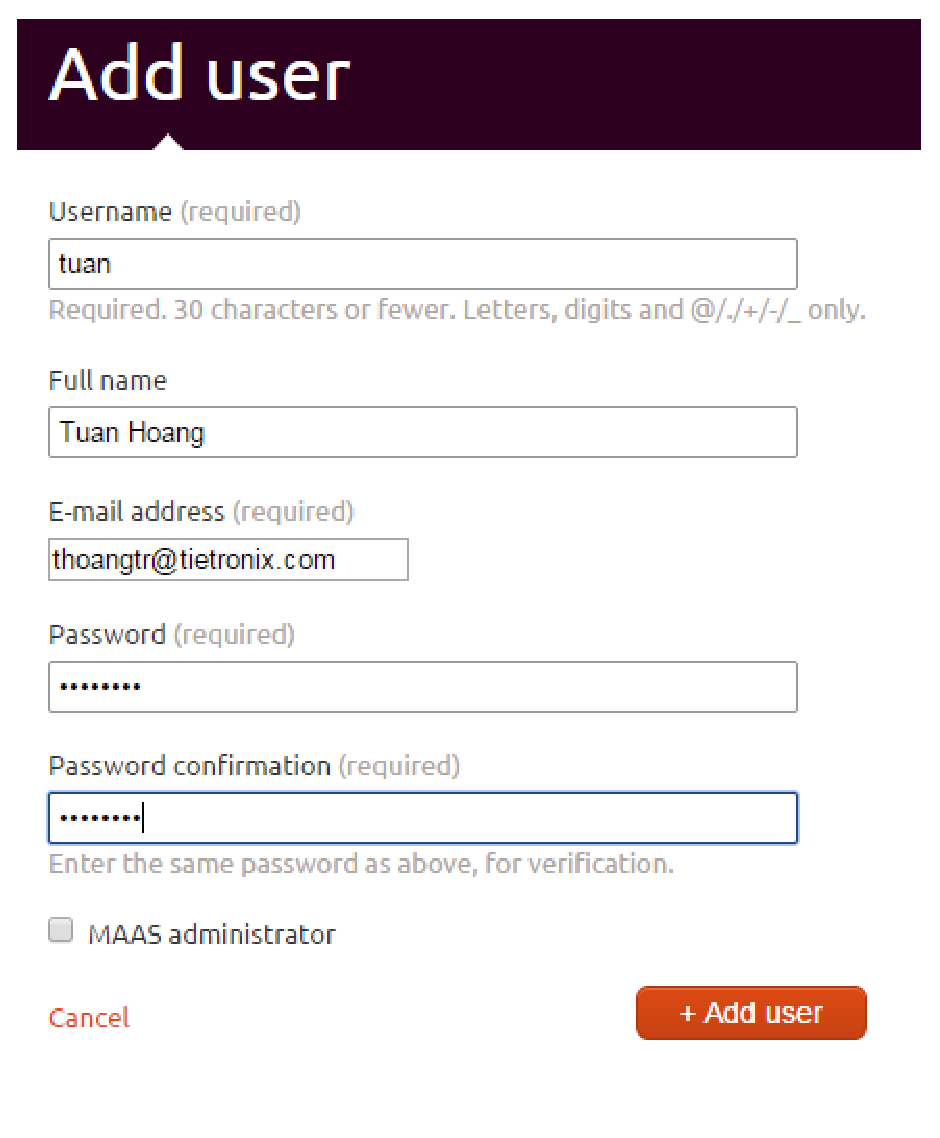
\includegraphics[height=4cm,
    angle=0]{./images/MaaS_new_user.eps}}
\caption{MaaS: create new user}
\label{fig:MaaS_new_user}
\end{figure}


\subsection{Deploy a service to MaaS node}
\label{sec:MaaS_deploy_service}

Once you have one or more MaaS node accepted in the MaaS cluster, you can deploy
services to that node, either manually or by using a tool like Juju.


\subsection{Troubleshoot}

\begin{enumerate}
  \item Update missing packages
\begin{verbatim}
sudo apt-get update --fix-missing
\end{verbatim}

  \item maas-dns depends on bind9
\begin{verbatim}
Errors were encountered while processing:
 bind9

dpkg: dependency problems prevent configuration of maas-dns:
 maas-dns depends on bind9; however:
  Package bind9 is not configured yet.

Errors were encountered while processing:
 bind9
 maas-dns
\end{verbatim}
A solution is to open these file 
\begin{verbatim}
/etc/bind/named.conf
/etc/bind/named.conf.options
\end{verbatim}
Search for and remove the line below
\begin{verbatim}
include "/etc/bind/maas/named.conf.options.inside.maas";
\end{verbatim} 
\url{https://bugs.launchpad.net/ubuntu/+source/maas/+bug/1346538}

  \item change MaaS server: If you change the ipaddress of your MaaS server you will need to run these
commands again.
\begin{verbatim}
sudo dpkg-reconfigure maas-region-controller

sudo dpkg-reconfigure maas-cluster-controller 
\end{verbatim}


  \item reinstall MaaS
\begin{verbatim}
sudo apt-get purge maas maas-dhcp maas-dns
sudo apt-get clean
sudo apt-get update
sudo apt-get upgrade
sudo apt-get install maas maas-dhcp maas-dns
\end{verbatim}
Make sure we reconfigure the MaaS servers
(Sect.\ref{sec:configure_MaaS_region-controller}).

\end{enumerate}


\url{https://maas.ubuntu.com/docs/troubleshooting.html}

\subsection{Building MaaS cluster using Virtual Machine}

REQUIREMENT:
\begin{itemize}
  \item A Ubuntu Desktop (host machine) with an external NIC card
  \item Install Virtual Machine Manager (VMM) on Ubuntu Desktop	
  \item Download Ubuntu Server 13.10 64-bit ISO image
\end{itemize}

In VMM, create your MaaS cluster
\begin{itemize}
  \item Edit/Connection 
  \item Select Virtual Networks tab
  \item Click '+' to add a network and go through wizzard setting
\begin{verbatim}
Name: maas
Network: new subnet (not conflict with physical network or any other 
         virtual networks)
Disable DHCP: 
NAT: do not bridge or host-only this network as we need to download PXE images
     later
\end{verbatim}  
\end{itemize}



Create a new virtual machine (MaaS region controller + cluster controller) via
VMM (use the downloaded ISO image)
\begin{itemize}
  \item CPU: 1, RAM: 1GB, Disk space: 30GB
  \item choose 'maas' network in Advanced Options
\begin{verbatim}
Virtual network 'maas': NAT
\end{verbatim}
  \item Check 'Set a fixed MAC address'
  
  \item Once Ubunt Server boot, choose 'Multiple server install with MaaS'. Walk
  through the setting just like
  Sect.\ref{sec:MaaS_install_region-controller_and_cluster-controller}	
  
  DHCP will fail, as we turned off VMM's DHCP server earlier. We need to
  configure the IP manually, use the IP in the range you selected for 'maas'
  network but do not use .1 (as it is reserved for VMM's {\bf virtual switch}).
  Use default NetMask (255.255.255.0) and Gateway (X.X.X.1) and name server
  entries provided by the installer. 
  
  When asked, select 'Create a new MaaS on this server'
  
\end{itemize}

Configure MaaS region controller (Sect.\ref{sec:configure_MaaS_region-controller})
\begin{itemize}
  \item Once the virtual machine is restarted, configure MaaS region controller
  (Sect.\ref{sec:configure_MaaS_region-controller})
\begin{verbatim}
sudo maas createsuperuser
\end{verbatim}

  Download boot images (Sect.\ref{sec:MaaS_download-boot-images}) to the MaaS
  region controller
\begin{verbatim}
sudo maas-import-pxe-files
\end{verbatim}

  \item Setup SSH tunnel
\begin{verbatim}
ssh -R 8080:localhost:80 <your-username>@<your-desktop>
\end{verbatim}

  \item Open the web browser (from host machine), and browse
\begin{verbatim}
http://locahost:8080/MAAS
\end{verbatim}
\end{itemize}

Configure MaaS cluster controller (Sect.\ref{sec:configure_MaaS-cluster-controller})
\begin{itemize}
  \item Configure the Network Interface from that the nodes can use: Broadcast,
  Router and IP range details.
  
  \item Configure the DHCP and DNS
\begin{verbatim}
sudo service maas-dhcp-server restart

sudo service maas-pserv restart
\end{verbatim}
\end{itemize}

Finally, we can add nodes to the MaaS cluster. There are two ways:
\begin{itemize}
  \item Create a new virtual machine instance, and add it to the 'maas' network
  (just like we install MaaS cluster controller)
  
  Use Ubuntu server ISO image, and select 'Multiple server install with MaaS'.
  Select 'Sepecify MaaS by name or address', and enter yhe MaaS controller
  information. Once complete, the node will shutdown.
  
  \item Create a new virtual machine instance and select the option 'Network
  Boot (PXE)'. This will cause this new VM to PXE boot from MaaS and enlist
  itself.
\end{itemize}

 Open the web browser, and browse MaaS Web UI.
 \begin{itemize}
   \item The status of the new machine will be 'Declared'
   \item Edit the node and choose 'PXE' as boot option for the declared node via
   VMM.
   
   MAAS handles virtual machine power management via the \verb!virsh! power
   management type. You have to manually configure the details for each node in
   order for MAAS to manage these virtual machines and turn them on/off
   automatically. 
   
   \item Commission the node by selecting ``Commission selected nodes'', the
   status will be 'Commissioning'. 
   
   Add \verb!use-fastpath-installer! tag to the node or use click the button
   \verb!Use the fast installer! to save some serious deployment time.
   
   \item Manually boot the node to complete the   commissioning process. The new
   status of the node should be ``Ready''. The node will shutdown again once it
   is in 'Ready' state.
 \end{itemize}
 New nodes can be added by repeating the above steps.
 
Once you have the MaaS clusters with a number of 'Ready' nodes, you can install
Juju.


\url{https://insights.ubuntu.com/2013/11/15/interested-in-maas-and-juju-heres-how-to-try-it-in-a-vm/}

\url{https://wiki.ubuntu.com/SecurityTeam/TestingMaaS}

\url{http://dinosaursareforever.blogspot.com/2014/06/manually-deploying-openstack-with.html}

\subsection{Power Type}
\label{sec:MaaS_powertype}

There are different methods to power on/off a machine remotely
(Sect.\ref{sec:power-remotely}). In this section, we discuss different devices
and/or methods that is supported by MaaS

\begin{verbatim}
Powertype: 
  - Wake-on-LAN
  - iLO4 Moonshot Chassis
  - Sentry Switch CDU
  - Digital Loggers, Inc. PDU
  - virsh (virtual systems)  
  - Moonshot HP iLO Chassis Manager
  - IPMI
  - SeaMicro 15000   (sm15k)
  - Cisco UCS Manager
  - Intel AMT
\end{verbatim}

The desktop motherboards have at least Wake-on-LAN powertype support. The server
motherboards can have different method to power on the machine, depending on the
vendor. 

\textcolor{red}{\bf virsh} (virtual machine only):
  \begin{itemize}
    \item \verb!virsh!: if you use virtual machine to setup as node, which needs
    3 information: Power ID, Address and Power type
    
    PowerID : \verb!sudo virsh list --all!
    
  \url{https://maas.ubuntu.com/docs/nodes.html} 
  \end{itemize}

\textcolor{red}{\bf Wake-on-LAN}: To enable Wake-on-LAN (WOL) on the remote
machine, this remote machine needs to have a NIC card with WOL enabled. There
are two scenarios: integrated NIC card, or external NIC card.
\begin{itemize}
  \item Integrated NIC card with the mainboard: 
the BIOS settings or from the command line or from
Windows setting. Here we only discuss the first method, as the machine has no
O/S installed yet.
\url{http://www.howtogeek.com/70374/how-to-geek-explains-what-is-wake-on-lan-and-how-do-i-enable-it/}
\begin{verbatim}
WOL (Wake-On-LAN) in S4
\end{verbatim}

  \item External NIC card: you will still have to configure your BIOS to allow
  devices to wake up your computer. Find the option to allow USB and/or PCI devices to wake-up the computer.
\begin{verbatim}
PCI Devices power on (BIOS/Advanced/ACPI Configuration/)
\end{verbatim}

PCI NICs sometimes require a cable connection to the power supply in order to
stay awake when the computer is off/asleep. Check your manual to see if yours
does and install if necessary.
\end{itemize}
\url{https://help.ubuntu.com/community/WakeOnLan}
%  Then you can test using another machine in the same network \begin{verbatim}
% wakeonlane 40:16:7e:a7:72:b1 \end{verbatim}

The code to call the command to power on/off remote machine for Wake-on-LAN
option is given in 
\begin{verbatim}
/etc/maas/templates/power/ether_wake.template
\end{verbatim}

As we can see in this code, MaaS 1.7 uses either \verb!etherwake! (which use
\verb!eth0! as the default interface) or \verb!wakeonlan! (which uses UDP via port) to boot the remote
nodes, if using power type Wake-on-LAN. However, these tools are not installed
by default, and are not dependencies of MaaS. Thus, it is important to install
these packages on MaaS cluster controller
\begin{verbatim}
apt-get install etherwake wakeonlan
\end{verbatim}
\begin{verbatim}
mac_address={{mac_address}}
power_change={{power_change}}

if [ "${power_change}" != 'on' ]
then
    echo "There is no way to power down a node through etherwake." >&2
    exit 1
elif [ -x /usr/bin/wakeonlan ]
then
    /usr/bin/wakeonlan $mac_address
elif [ -x /usr/sbin/etherwake ]
then
    /usr/sbin/etherwake $mac_address
else
    echo "No wakeonlan or etherwake program found." >&2
fi

exit 0
\end{verbatim}
However, there are a number of reason to change the script and modify
\verb!/etc/sudoers.d/99-maas-sudoers! file
\begin{enumerate}
  \item \verb!wakeonlan! does not allow us to change the Interface, and the
  signal transmission via UDP is not reliable.

It is recommended NOT to install \verb!wakeonlan! as we can not boot remotely
using this method when there is more than one Interface. Also, it is recommended to
adjust the file content and move the condition for \verb!etherwake! before
\verb!wakeonlan!.

   \item   Also, making sure \verb!eth0! is the interface to the MaaS cluster region. 
However, since Ubuntu 14.04, \verb!eth0! is no longer being used but \verb!p2p1!
or \verb!p3p1! instead

We need to mofidy and add the correct interface via the \verb!-i!
option of \verb!etherwake! command.
   
   \item \verb!etherwake! requires root or \verb!sudo!. 
   
As this command is run  by MaaS admin user, not the machine admin user, so we
need to run this command as \verb!sudo! and put the command 
\begin{verbatim}
maas ALL= NOPASSWD: /usr/sbin/etherwake
\end{verbatim}
to the content of \verb!/etc/sudoers.d/99-maas-sudoers! file (Sect.\ref{sec:sudo})

Example: Here the machine user that MaaS user is named \verb!maas!
(Sect.\ref{sec:specify_machine-user_MaaS-use}) 

{\tiny
\begin{verbatim}
maas ALL= NOPASSWD: /usr/sbin/service maas-dhcpd restart
maas ALL= NOPASSWD: /usr/sbin/service maas-dhcpd6 restart
maas ALL= NOPASSWD: /usr/sbin/service maas-dhcpd stop
maas ALL= NOPASSWD: /usr/sbin/service maas-dhcpd6 stop
maas ALL= NOPASSWD: /usr/sbin/maas-provision
maas ALL= NOPASSWD: SETENV: /usr/sbin/maas-import-pxe-files, /usr/sbin/tgt-admin, /usr/bin/uec2roottar
maas ALL= NOPASSWD: /usr/sbin/etherwake
\end{verbatim}
} 
\end{enumerate}
\url{http://askubuntu.com/questions/504452/node-in-maas-not-waking-up-on-lan}

SUMMARY: new content
\begin{verbatim}
mac_address={{mac_address}}
power_change={{power_change}}

if [ "${power_change}" != 'on' ]
then
    echo "There is no way to power down a node through etherwake." >&2
    exit 1
elif [ -x /usr/sbin/etherwake ]
then
    sudo /usr/sbin/etherwake -i p3p1 $mac_address
elif [ -x /usr/bin/wakeonlan ]
then
    /usr/bin/wakeonlan $mac_address
else
    echo "No wakeonlan or etherwake program found." >&2
fi

exit 0
\end{verbatim}

\url{/etc/maas/templates/power/ether_wake.template}
 
\textcolor{red}{\bf Intel AMT}: It requires the processor and motherboard to
have Intel vPro feature, which can be checked by looking for vPro sticker.
 Another option is to look for an option to enable AMT (or to enable CTRL P
 prompt) in the BIOS setting. There is also a tool
 \url{https://communities.intel.com/docs/DOC-2060}
Intel AMT SDK to be used for software that interact with Intel AMT:
\url{https://software.intel.com/en-us/articles/download-the-latest-intel-amt-software-development-kit-sdk}

\textcolor{red}{\bf SeaMicro SM15000 Fabric Servers}: This AMD product provides
an equivalent 32 1RU dual socket servers, massive bandwidth with 64 sockets
AMD's octal core Opteron or Intel quad-core Xeon
\url{http://www.seamicro.com/sm15000}
\begin{verbatim}
local/etc/maas/templates/power/sm15k.template
\end{verbatim}
Code to support the ability to query the power status of sm15k using REST API
v2.0
\url{https://code.launchpad.net/~blake-rouse/maas/sm15k-query}
\url{https://bugs.launchpad.net/maas/+bug/1326485}


\textcolor{red}{\bf Cisco UCS Manager}: 
\begin{verbatim}
local/etc/maas/templates/power/ucsm.template:
\end{verbatim}

\subsection{User account}
\label{sec:MaaS_user-account}

MaaS use Django to manage user accounts.

\textcolor{red}{\bf Admin accounts}: You can create as many admin account if you
want, requirement
\begin{itemize}
  \item different email
\end{itemize} 
using the command below on the region controller server
\begin{verbatim}
// MaaS 1.4
sudo maas createsuperuser

// MaaS 1.5+
sudo maas-region-admin createadmin --username=root --email=MYEMAIL@EXAMPLE.COM
\end{verbatim}
You may also use a different username for your administrator account, but "root"
is a common convention and easy to remember. The command will prompt for a password to assign to the new user.

Example: error
\begin{verbatim}
django.db.utils.IntegrityError: duplicate key value violates unique constraint "auth_user_email_key"
DETAIL:  Key (email)=(thoangtr@tietronix.com) already exists.

\end{verbatim}

\section{Hack MaaS}

\url{https://maas.ubuntu.com/docs/hacking.html}

\subsection{Download and Build MaaS from source}

\url{https://maas.ubuntu.com/docs/hacking.html}

We need to download latest source code from launchpad using \verb!bzr! tool
\begin{verbatim}
sudo apt-get install bzr

bzr branch lp:maas/1.7 maas && cd maas
\end{verbatim}

MAAS depends on Postgres 9.1, RabbitMQ, Apache 2, daemontools, pyinotify, and
many other packages
\begin{verbatim}
make install-dependencies

 //remove some packages that no longer need
sudo apt-get autoremove
\end{verbatim}

\subsection{Query power type}
\label{sec:query_powertype}

The different schemas shown in the Web UI is in the source file
\begin{verbatim}
local/src/provisioningserver/power_schema.py
\end{verbatim}
with example Wake-on-LAN option
\begin{verbatim}
JSON_POWER_TYPE_PARAMETERS = [
    {
        'name': 'ether_wake',
        'description': 'Wake-on-LAN',
        'fields': [
            make_json_field(
                'mac_address', "MAC Address", field_type='mac_address'),
        ],
    },

\end{verbatim}

Source 
\begin{verbatim}
 src/provisioningserver/rpc/power.py
\end{verbatim}
At MaaS 1.7, the following power types are supported to query
\begin{verbatim}
QUERY_POWER_TYPES = ['amt', 'ipmi', 'mscm', 'sm15k', 'ucsm', 'virsh']
\end{verbatim}

The code to really do the query is 
\begin{verbatim}
from provisioningserver.power.poweraction import (
    PowerAction,
    PowerActionFail,
    )
\end{verbatim}
in the file
\begin{verbatim}
 src/provisioningserver/power/poweraction.py
\end{verbatim}

\subsection{Specify machine users and groups that MaaS uses}
\label{sec:specify_machine-user_MaaS-use}

MaaS uses Django and Django needs to perform some commands, e.g. wake up a
remote machine, as some machine user. This information about the machine user
and its group are defined in 
\begin{verbatim}
src/maas/settings.py
\end{verbatim}

When deployed, it is stored in
\begin{verbatim}
/etc/maas/maas_local_settings.py
\end{verbatim}


Example:
\begin{verbatim}
DATABASES = {
    'default': {
        # 'postgresql_psycopg2', 'postgresql', 'mysql', 'sqlite3' etc.
        'ENGINE': 'django.db.backends.postgresql_psycopg2',
        'NAME': 'maasdb',
        'USER': 'maas',
        'PASSWORD': 'g9jsjAO7Non3',
        'HOST': 'localhost',
        'OPTIONS': {
            'isolation_level': ISOLATION_LEVEL_READ_COMMITTED,
        },
    }
}
\end{verbatim}

Current, \verb!maas! is the machine user that MaaS uses. However, by default,
there is no home directory created for this user, we can do that

\begin{verbatim}
sudo mkdir /home/maas

sudo chown maas:maas /home/maas

 # add login shell as well
sudo chsh -s /bin/bash maas
\end{verbatim}





\section{Juju (Ensemble)}
\label{sec:Juju}

Juju (formally known as Ensemble) packages the intelligence of installing,
configuring and managing services. It is likened to APT tool for a given cloud
provider, i.e. helping to install something on multiple machines easily. 

With Juju, different authors are able to create \verb!service formulas!, called
\verb!charms!, independently, and make those services coordinate their
communication and configuration through a simple protocol.
Juju includes a collection \verb!charms! that let you deploy whatever services
you want in Juju.  A \verb!charm! tells us how to manage a service. A service
can be (1) mysql database, (2) wordpress. After the services are deployed, Juju
can define the relations between them (e.g. wordpress needs mysql), and expose
the services to the outside world. 
Juju thus is called {\bf service orchestration}.
\url{http://askubuntu.com/questions/80330/what-is-a-juju-charm}

\begin{itemize}
  \item  an automation layer (with an API) is deployed on top of a data-center
  
  With an API call, a click of button or executing a command, servers can be
  created or destroyed, storage can spring up to existence and various virtual
  networks are created to service the virtual datacenter just created. 
  
  
\end{itemize}
A potential solution to that is PaaS cloud environments, that try to solve the
issue by offering runtime environments that contain standard configurations for
common components and frameworks (databases, application servers... and so on). 

A collection of charms that are designed to work together is called a
\verb!Bundle!. Both charms and bundles are included in what we collectively call
The Charm Store. \url{https://juju.ubuntu.com/docs/authors-charm-store.html}


There are different cloud provider (e.g. Amazon EC2, Microsoft Azure, etc.)


Example: Let's deploy a multi-tier LAMP application to the cloud  Amazon EC2
cloud, connect all the pieces together and see how it fares.

\subsection{Charm}
\label{sec:Charm}

\verb!Charm! is a distribution of charms for juju
\url{https://launchpad.net/charm-tools}

\begin{verbatim}
sudo add-apt-repository ppa:juju/stable
sudo apt-get install charm-tools
\end{verbatim}
which installs
\begin{verbatim}
charm-tools python-charmworldlib python-cheetah python-markdown
\end{verbatim}

The many tools provided by Charm is
\url{https://juju.ubuntu.com/docs/commands.html}
\begin{verbatim}
juju help commands
\end{verbatim}

\begin{enumerate}
  \item \verb!action!:
  \item \verb!add-machine! : start a new, empty machine
  
  we can add a container to a machine
  \item \verb!add-relation!: add a relation between 2 services
  
  \item \verb!add-unit! : 
  
  \item \verb!api-endpoints! 
  
  \item \verb!authorised-keys! : 
  
  \item \verb!backups! : 
  
  \item \verb!sync-tools! : copy tools from the official tool store into a local
  environment

We also need tools for the public release 
\begin{verbatim}
juju sync-tools
\end{verbatim}
This copies the Juju tools tarball from the official bucket into your
environment. This is generally done when you want Juju to be able to run without
having to access Amazon.
Sometimes this is because the environment does not have public access, and
sometimes you just want to avoid having to access data outside of the local
cloud. 
\url{http://askubuntu.com/questions/285395/how-can-i-copy-juju-tools-for-use-in-my-deployment}


\end{enumerate}



\subsection{Install}
\label{sec:Juju_install}

Juju server runs on Ubuntu server or Max OS X or Windows.
\url{https://juju.ubuntu.com/install/}
\begin{verbatim}
sudo apt-get install software-properties-common
sudo add-apt-repository ppa:juju/stable

sudo apt-get update && sudo apt-get install juju-core
\end{verbatim}


Now, we need to create a new Juju environment.  On the cluster controller, we
run
\begin{verbatim}
$> juju generate-config

A boilerplate environment configuration file has been written to /home/tietronix/.juju/environments.yaml.
Edit the file to configure your juju environment and run bootstrap.
\end{verbatim}
which generates the configuration file \verb!~/.juju/environments.yaml!
(Sect.\ref{sec:juju/environments.yaml}).

\subsection{bootstrap node}
\label{sec:juju_bootstrap_node}

Once you install Juju (Sect.\ref{sec:Juju_install}), before we can install any
service, the first thing an juju environment needs is a bootstrap node. For now,
it needs a dedicated node.  This is the node that is used to manage the
Juju environment.

Juju will pick out a node in the cluster and make it as the bootstrap node. That
explains why we need at least two nodes: MaaS cluster controller and juju
bootstrap node.

Commands: 
\begin{verbatim}
#### which randomly select a node to make the bootstrap node
$> juju bootstrap -e maas --debug

// juju 1.14.0+
$> juju bootstrap --upload-tools


#### which select a node to do the bootstrap
juju bootstrap --to <hostname>
juju add-machine <hostname>
\end{verbatim}

The bootstrap node (or master node) might take long time, as it has to
completely install Ubuntu and Juju on it and reboot before it'll be  available
for use.


The output
\begin{verbatim}
$> juju bootstrap

WARNING ignoring environments.yaml: using bootstrap config in file "/home/tietronix/.juju/environments/maas.jenv"
Launching instance
WARNING picked arbitrary tools &{1.20.14-trusty-amd64 http://192.168.1.10/MAAS/api/1.0/files/?key=d37a134a-a72b-11e4-9805-40167ea604f1&op=get_by_key ad7360aa5512b8d7cc1ad0ceb223bd9a1c8f5c6b0b131b5a3bd8fde623b85585 8130261}
 - /MAAS/api/1.0/nodes/node-9fd0a794-a680-11e4-89c4-40167ea604f1/
Waiting for address
Attempting to connect to hadu02.maas:22
Attempting to connect to hadu02.maas:22
Attempting to connect to 192.168.1.2:22
@@@@@@@@@@@@@@@@@@@@@@@@@@@@@@@@@@@@@@@@@@@@@@@@@@@@@@@@@@@
@    WARNING: REMOTE HOST IDENTIFICATION HAS CHANGED!     @
@@@@@@@@@@@@@@@@@@@@@@@@@@@@@@@@@@@@@@@@@@@@@@@@@@@@@@@@@@@
IT IS POSSIBLE THAT SOMEONE IS DOING SOMETHING NASTY!
Someone could be eavesdropping on you right now (man-in-the-middle attack)!
It is also possible that a host key has just been changed.
The fingerprint for the ECDSA key sent by the remote host is
51:11:c7:7b:a1:4a:80:eb:33:0a:ae:96:ff:5b:4f:bb.
Please contact your system administrator.
Add correct host key in /home/tietronix/.ssh/known_hosts to get rid of this message.
Offending ECDSA key in /home/tietronix/.ssh/known_hosts:1
  remove with: ssh-keygen -f "/home/tietronix/.ssh/known_hosts" -R 192.168.1.2
Keyboard-interactive authentication is disabled to avoid man-in-the-middle attacks.
sudo: unable to resolve host hadu02
Logging to /var/log/cloud-init-output.log on remote host
Running apt-get update
Running apt-get upgrade
Installing package: git
Installing package: curl
Installing package: cpu-checker
Installing package: bridge-utils
Installing package: rsyslog-gnutls
Fetching tools: curl -sSfw 'tools from %{url_effective} downloaded: HTTP %{http_code}; time %{time_total}s; size %{size_download} bytes; speed %{speed_download} bytes/s ' --retry 10 -o $bin/tools.tar.gz 'http://192.168.1.10/MAAS/api/1.0/files/?key=d37a134a-a72b-11e4-9805-40167ea604f1&op=get_by_key'
Bootstrapping Juju machine agent
Starting Juju machine agent (jujud-machine-0)
\end{verbatim}

NOTICE: the error
\begin{verbatim}
sudo: unable to resolve host hadu02
\end{verbatim}
When using a third party tool such as juju it will need to be able to resolve
the hostnames that the MAAS API returns to it. In order for this to happen,
client-side DNS must be configured to point to MAAS's DNS server
(Sect.\ref{sec:MaaS_maas-dns}).


Otherwise you can get errors
\begin{verbatim}
Launching instance
WARNING picked arbitrary tools &{1.20.11-precise-amd64 https://streams.canonical.com/juju/tools/releases/juju-1.20.11-precise-amd64.tgz 196a1348755f3ce869ce1319995d2d6b672809e165d87987dc5c12828c228de8 8112417}
ERROR bootstrap failed: cannot start bootstrap instance: gomaasapi: got error back from server: 400 BAD REQUEST ({"distro_series": ["'precise' is not a valid distro_series.  It should be one of: '', 'ubuntu/trusty'."]})
Bootstrap failed, destroying environment
ERROR cannot start bootstrap instance: gomaasapi: got error back from server: 400 BAD REQUEST ({"distro_series": ["'precise' is not a valid distro_series.  It should be one of: '', 'ubuntu/trusty'."]})

\end{verbatim}

Once a bootstrap node is setup, we can check
\begin{verbatim}
$> juju status

environment: maas
machines:
  "0":
    agent-state: started
    agent-version: 1.20.14
    dns-name: hadu02.maas
    instance-id: /MAAS/api/1.0/nodes/node-9fd0a794-a680-11e4-89c4-40167ea604f1/
    series: trusty
    hardware: arch=amd64 cpu-cores=8 mem=16384M
    state-server-member-status: has-vote
\end{verbatim}

Now, it's possible to deploy any charm (i.e. service).
Note that each charm runs on its own host, so each deployment will actually take
as long as it took to bootstrap.
\begin{itemize}
  \item mysql
  
\begin{verbatim}
juju deploy mysql
\end{verbatim}

  \item wordpress
\begin{verbatim}
$ juju deploy wordpress
$ juju add-relation wordpress mysql
$ juju expose wordpress
$ juju status
\end{verbatim}
\url{http://maas.ubuntu.com/docs/juju-quick-start.html}

\end{itemize}


\subsection{.juju/environments.yaml}
\label{sec:juju/environments.yaml}

NOTE: \verb!#! is used to indicate a comment-line.  There are several
informations that need to be filled in by user, especially those in brackers
\verb!<brackets>!. Optional attributes are commented out, depending on what
service you want to deploy, e.g. MaaS (Sect.\ref{sec:MaaS_Juju}), Amazon EC2, \ldots


This environment will provide a new server with an Ubuntu cloud O/S image
on-demand, e.g Amazon EC2, HP Cloud, OpenStack installation, on your local machine.
Each environment must specify at least the following information
\begin{itemize}
  \item name (to identify the environment), e.g. myenv2
  \item type (to specify the provider), e.g. \verb!ec2!, \verb!maas!,
  \verb!openstack!, \verb!manual!, \verb!local!, \verb!joyent!, \verb!azure!
  
\begin{verbatim}
myenv2:
  type: ec2
\end{verbatim}
 \end{itemize}
and some other provider-specific information.

There can be multiple environments, the environment to be used following the
given descending order
\begin{enumerate}
  \item specify via the \verb!-e! or \verb!--environment! command line parameter
\begin{verbatim}
$> juju add-unit -e myenv2 myservice
\end{verbatim}
  
  \item if the above is not given, it check the environment variable
  \verb!JUJU_ENV!
  
  \item if the above is not defined neither, it check the switch command
\begin{verbatim}
juju switch myenv
\end{verbatim}

  \item if none of the above is used, it looks into the configuration file 
 \verb!default:! tag.
\begin{verbatim}
default: amazon
\end{verbatim}

\end{enumerate}

Example:
\begin{verbatim}
default: amazon
 
environments:
   openstack:
      type: openstack
\end{verbatim}


\url{https://maas.ubuntu.com/docs/juju-quick-start.html}

On the MaaS cluster controller, check the version so that you know the commands
to use
\begin{verbatim}
$> juju --version

1.20.14-trusty-amd64
\end{verbatim}

What we need
\begin{itemize}
  \item SSH key-pair (Sect.\ref{sec:passwordless-ssh})
  
NOTE: \url{https://maas.ubuntu.com/docs/nodes.html} 
  
  \item configure Juju to use the cloud provider: we can specify multiple
  environments in which to deploy (e.g. Amazon AWS, HP Cloud, OpenStack, Azure,
  MaaS, Local and Manual providers).
  
  
To list the existing configuration
\begin{verbatim}
$> juju generate-config --show
\end{verbatim}
\end{itemize}


\subsection{Maas + JuJu}
\label{sec:MaaS_Juju}

MaaS only allows you to add/remove a physical machine easily. However, it does
not install any service at all on these machine. To do that, we need Juju.
Before we continue, make sure MaaS cluster has at least 2 nodes enlisted with
it (Sect.\ref{sec:MaaS_node_install} or Sect.\ref{sec:MaaS_node_virtual}). 

Now, we install Juju on the machine where MaaS cluster controller is installed
and bootstrap a new environment follow the above steps
(Sect.\ref{sec:Juju_install}). Edit the file
\begin{verbatim}
~/.juju/environment.yaml
\end{verbatim}

and change to \verb!maas! as the default cloud service (look at the
beginning of the file)
\begin{verbatim}
  // change to 'maas', instead of 'amazon'
default: amazon 
\end{verbatim}

Then, notice the section \verb!type: maas! in \verb!~/.juju/environment.yaml!
file
\begin{verbatim}
# juju: environments
environments:
  maas:
    type: maas
    maas-server: 'http://localhost/MAAS'
    maas-oauth: '${maas-api-key}'
    admin-secret: 'nothing'
    // default series is 'precise' (12.04), but you can change
    // to 'trusty' (Ubuntu 14.04)
    default-series: precise
    
## add your SSH key to the configuration file
## so that MaaS can add them to the new node    
 authorized-keys-path: ~/.ssh/id_rsa.pub     
\end{verbatim}
with the content (substitute the \verb!${maas-api-key}! with MAAS API key). 
You need API key from MaaS so that Juju client can access it. One hard rule is
to use a different API key for each Juju environment you set up within a single
MaaS cluster.
  
Juju automatically detect MaaS networks, recognize physical and virtual networks
on each machine. Just run, \verb!juju status! to show the discovered network.

 When you run \verb!juju status!, you may get the error
\begin{verbatim}
$> juju status

ERROR Unable to connect to environment "amazon".
Please check your credentials or use 'juju bootstrap' to create a new environment.

Error details:
control-bucket: expected string, got nothing

\end{verbatim}




\subsection{MaaS/Juju and OpenStack}
\label{sec:MaaS_OpenStack}

Originally, MaaS is designed to help deploy Ubuntu O/S easily to a new node.
Recently, it has been designed to use OpenStack and support deploying other
operating systems.
Here, we discuss how to use OpenStack with MaaS

\url{http://www.ubuntu.com/download/cloud}

Ubuntu Cloud Images are pre-installed disk images that have been customized by
Ubuntu engineering to run on cloud-platforms such as Amazon EC2, Openstack, Windows and LXC.
\url{https://cloud-images.ubuntu.com/}

\url{http://askubuntu.com/questions/476371/how-do-i-use-maas-to-prepare-to-install-openstack}

It's assumed the user has sufficient number of nodes available in MAAS.



\subsection{MaaS/Juju + Hadoop}
\label{sec:MaaS_Hadoop}




\url{http://www.zdnet.com/article/ubuntu-chases-enterprise-cloud-with-server-14-04-release/}

\section{Eucalyptus}
\label{sec:Eucalyptus}

Eucalyptus is an open-source software for building Amazon Web
Service (AWS-compatible) private/hybrid clouds. It is an IaaS product and allows
us to provision the collection of resources (both compute and storage) on an as-needed basis.
\url{https://www.eucalyptus.com/docs/eucalyptus/4.0.2/index.html\#user-guide/index.html}

Eucalyptus is the acronym for Elastic Utility Computing Architecture for Linking
Your Programs To Useful Systems. Eucalyptus Systems announced a formal agreement
with AWS in March 2012 to maintain compatibility. In September 2014, Eucalyptus
was acquired by Hewlett-Packard.

The software development had its roots in the Virtual Grid Application
Development Software project, at Rice University and other institutions from
2003 to 2008. 

Eucalyptus commands can manage either Amazon or Eucalyptus instances,
Fig.\ref{fig:Eucalyptus}. Users can also move instances between a Eucalyptus
private cloud and the Amazon Elastic Compute Cloud to create a hybrid cloud. Hardware virtualization isolates
applications from computer hardware details.


\begin{figure}[hbt]
  \centerline{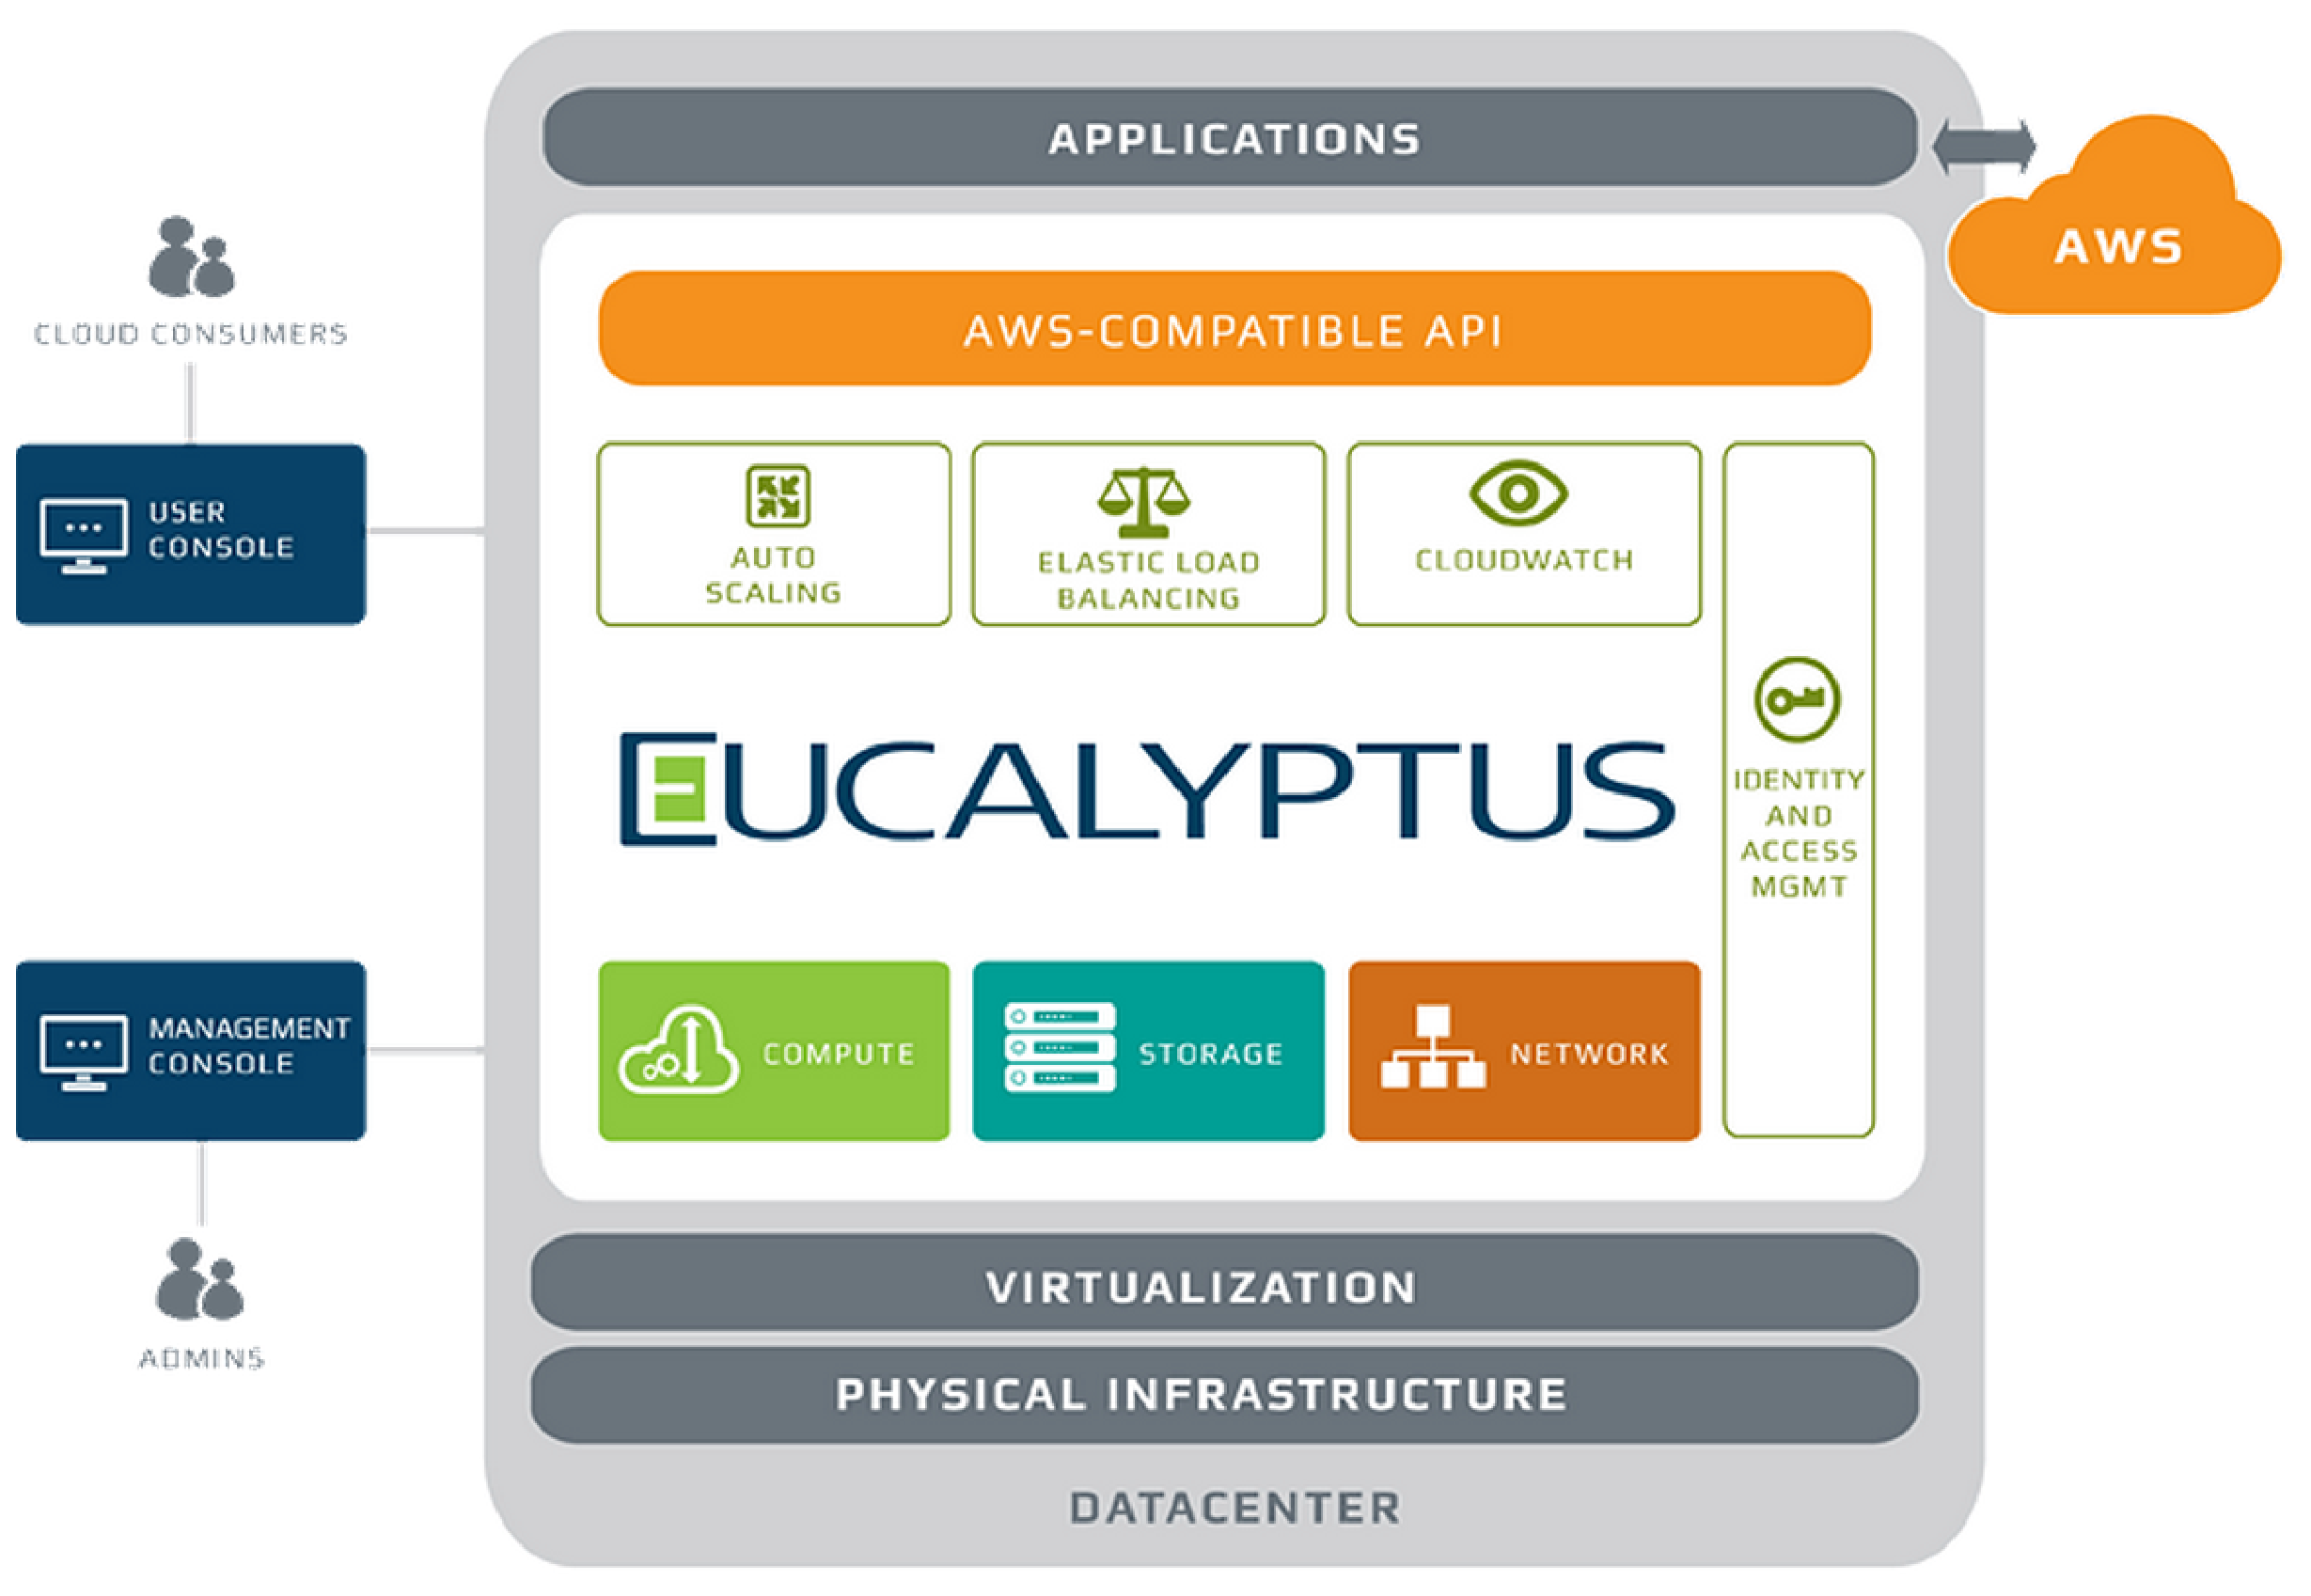
\includegraphics[height=6cm,
    angle=0]{./images/Eucalyptus.eps}}
\caption{Eucalyptus}
\label{fig:Eucalyptus}
\end{figure}

Walrus, also written in Java, is the Eucalyptus equivalent to AWS Simple Storage
Service (S3). Walrus offers persistent storage to all of the virtual machines in
the Eucalyptus cloud and can be used as a simple HTTP put/get storage as a
service solution.

\url{http://en.wikipedia.org/wiki/Eucalyptus_(software)#Software_architecture}

\section{squashfs}
\label{sec:squashfs}

